\documentclass[lettersize,journal]{IEEEtran}
\usepackage{amsmath,amsfonts}
\usepackage{algorithmic}
\usepackage{algorithm}
\usepackage{array}
\usepackage[caption=false,font=normalsize,labelfont=bf,textfont=normalfont]{subfig}
\usepackage{textcomp}
\usepackage{stfloats}
\usepackage{url}
\usepackage{verbatim}
\usepackage{graphicx}
\usepackage{cite}
\usepackage{booktabs}
\usepackage{multirow}
\usepackage{tikz}
\usetikzlibrary{shapes.geometric,arrows.meta,positioning,fit,backgrounds,calc}
\hyphenation{op-tical net-works semi-conduc-tor IEEE-Xplore}

\begin{document}

% ============================================================
%  TITLE
% ============================================================
\title{A Risk-Weighted Active Learning Framework for Annotation-Constrained UAV Multispectral Anomaly Detection}

% ============================================================
%  AUTHORS  (fill in affiliations / ORCID before submission)
% ============================================================
\author{Ali G{\"u}ne\c{s},~\IEEEmembership{Member,~IEEE,}
        Author Two,~\IEEEmembership{Member,~IEEE,}
        and~Author Three% <-this % stops a space
\thanks{Manuscript received XX Month 2025.}%
\thanks{A.~G{\"u}ne\c{s} is with the Faculty of Engineering and
Natural Sciences, Department of Software Engineering, Atlas University,
Istanbul 34406, Turkey (e-mail: ali.gunes@atlas.edu.tr).
Author Two and Author Three are with the Department of Electronics and
Computer Science, Universidade de Santiago de Compostela,
15782 Santiago de Compostela, Spain (e-mail: author@usc.es).}%
\thanks{This work was supported in part by [GRANT INFO].}}

\markboth{IEEE Journal of Selected Topics in Applied Earth Observations
and Remote Sensing}%
{G{\"u}ne\c{s} \MakeLowercase{\textit{et al.}}: Risk-Weighted Active Learning for UAV Anomaly Detection}

\IEEEpubid{0000--0000/00\$00.00~\copyright~2025 IEEE}

\maketitle

% ============================================================
%  ABSTRACT
% ============================================================
\begin{abstract}
This paper proposes a cost-sensitive active learning (cAL) framework
for UAV multispectral environmental anomaly detection. Unlike
conventional active learning methods that primarily optimize global
classification accuracy, the proposed framework explicitly penalizes
missed anomalies through a configurable risk coefficient~$r^{+}$.
The method integrates a cost-sensitive support vector machine (cSVM),
risk-sensitive margin uncertainty sampling, and kernel $k$-means
diversity filtering to select informative and non-redundant
superpixels under limited annotation budgets. Experiments on four
UAV multispectral riparian scenes from the Galician Rivers
Multispectral Anomaly Detection Dataset show that the proposed
strategy substantially reduces false negatives and risk-weighted
misclassification cost compared with random sampling, standard
margin-based active learning, and an uncertainty-diversity baseline.
At the highest risk level ($r^{+}=4$), the aggregate false-negative
rate decreases from $0.223$ under standard active learning to
$0.076$, and anomaly recall increases from $0.777$ to $0.924$,
corresponding to a $66.1\%$ reduction in missed anomalies. These
results demonstrate that incorporating operational risk into both
model training and query selection is effective for reducing missed
environmental anomalies in annotation-constrained UAV monitoring
workflows.
\end{abstract}

\begin{IEEEkeywords}
Active learning, cost-sensitive learning, UAV multispectral imagery,
environmental anomaly detection, riparian monitoring, false negative
reduction, support vector machine, kernel $k$-means, watershed
management.
\end{IEEEkeywords}

% Push right column down enough to clear the IEEEpubid watermark
\IEEEpubidadjcol

% ============================================================
%  I. INTRODUCTION
% ============================================================
\section{Introduction}
\IEEEPARstart{R}{iparian} and riverine ecosystems perform vital ecological
services, including nutrient cycling, flood attenuation, soil stabilisation,
and the provision of habitat corridors for both aquatic and terrestrial
species~\cite{arguello2021watershed}. Human encroachment---through road
construction, illegal building, drainage modification, and invasive
species---poses a persistent and escalating threat to these habitats.
Timely detection of such anomalies is a precondition for effective
watershed management, yet traditional in-situ surveys are expensive, slow,
and hazardous in remote or densely vegetated terrain.
Uncrewed aerial vehicles (UAVs) equipped with multispectral sensors offer
an attractive alternative: they combine the high spatial resolution needed
to resolve small structures with the spectral discriminability required to
separate anthropogenic features from dense riparian vegetation
\cite{colomina2014uav,arguello2021watershed}.

Despite the potential of UAV multispectral imagery for environmental
monitoring, two compounding challenges limit its operational deployment.
First, the annotation burden is substantial. Supervised classifiers require
expert-labelled training examples, and labelling superpixels or pixel
patches across large-format multispectral images demands significant domain
expertise and time. Active learning (AL) addresses this constraint by
iteratively selecting the most informative unlabelled samples for human
review~\cite{settles2012active,tuia2011survey}, reducing the annotation
budget needed to achieve a target detection performance.

Second, and more fundamentally, misclassification errors in environmental
monitoring carry asymmetric consequences. A false negative---a missed
anomaly---allows a threatening structure or pollution event to persist,
potentially triggering irreversible ecological degradation. A false
positive, by contrast, incurs only the manageable cost of a follow-up
field inspection. Standard active learning methods optimise symmetric
objectives such as classification accuracy or ROC-AUC, which treat both
error types equally~\cite{crawford2013active}. In doing so, they implicitly
accept high false-negative rates whenever the anomaly class is rare,
precisely the setting that is most operationally dangerous.

This paper addresses this gap by introducing a \emph{cost-sensitive active
learning} (cAL) framework that incorporates the asymmetric cost of missed
anomalies at every stage of the learning pipeline. A single, configurable
risk coefficient~$r^{+}$ controls the false-negative penalty in (i) the
classifier objective, through a class-weighted support vector machine
(cSVM); (ii) the query strategy, through a risk-sensitive margin
uncertainty score; and (iii) the evaluation metric, through the
risk-weighted cost~$C(r^{+})$. Kernel $k$-means diversity filtering
prevents redundant selections, ensuring that the annotation budget is
spread across spectrally distinct regions of the feature space. The
proposed approach is evaluated on the Galician Rivers Multispectral
Anomaly Detection Dataset~\cite{galicianriversaddataset}, which comprises
four large-format UAV scenes with ground-truth anomaly masks and realistic
class imbalance (3\%--13\% anomaly prevalence).

The main contributions of this paper are as follows:
\begin{enumerate}
  \item A cost-sensitive active learning framework for UAV multispectral
        riparian anomaly detection that unifies risk-weighted training,
        risk-sensitive querying, and risk-sensitive evaluation under a
        single risk coefficient~$r^{+}$.
  \item A risk-weighted evaluation criterion,
        $C(r^{+}) = (r^{+}\,\mathrm{FN}+\mathrm{FP})/N\times 100$,
        that directly reflects the operational cost of missed environmental
        anomalies.
  \item A two-stage query strategy combining risk-sensitive margin
        uncertainty with kernel $k$-means diversity filtering in the
        RBF-induced feature space.
  \item A 19-dimensional superpixel feature representation combining
        per-band statistics, vegetation indices (NDVI, NDRE, ExG, EVI,
        BNDVI), spectral band ratios, and a Mahalanobis-like spectral
        anomaly score, with an ablation study quantifying the contribution
        of each feature group.
  \item A comprehensive empirical comparison against random sampling,
        standard margin-based AL, and an uncertainty-diversity baseline
        across four UAV scenes and four risk levels, demonstrating a
        $66.1\%$ reduction in missed anomalies at the highest risk
        level ($r^{+}=4$).
\end{enumerate}

The remainder of this paper is organised as follows.
Section~II reviews related work on active learning in remote sensing,
cost-sensitive learning, and multispectral anomaly detection.
Section~III presents the dataset, the proposed cAL framework, and the
experimental setup.
Section~IV reports experimental results.
Section~V discusses implications and limitations.
Section~VI concludes.

% ============================================================
%  II. RELATED WORK
% ============================================================
\section{Related Work}

\subsection{Active Learning in Remote Sensing}

Pool-based active learning (AL) iteratively selects unlabelled samples from a
fixed pool for oracle annotation~\cite{settles2012active}. Uncertainty
sampling---querying the sample on which the current classifier is least
confident---is among the simplest and most effective strategies.
Margin-based uncertainty, defined as the absolute distance of a sample
from the SVM decision boundary, is a widely used instantiation that
selects the sample with the smallest signed margin~\cite{tong2001support}.
Support vector machines (SVMs) are particularly well-suited to AL because
the margin geometry provides a natural uncertainty measure and the
decision boundary is updated efficiently as new labels are
added~\cite{mountrakis2011svms,chang2011libsvm}.
For remote sensing data, where label acquisition is expensive, AL has been
applied to hyperspectral image classification~\cite{li2013rs}, land-cover
mapping, change detection, and scene recognition, often achieving
supervised-level performance with a small fraction of the full labelling
budget~\cite{tuia2011survey,crawford2013active,guo2023active,gunes2026geoai}.
Recent work has extended AL to deep learning models through
gradient-based and core-set query strategies~\cite{ash2020deep,sener2018active},
but SVM-based approaches retain practical advantages in low-annotation
regimes where deep networks are prone to overfitting.

A key challenge in applying AL to remote sensing is the large pool size
and the high spatial autocorrelation of image data. Querying spatially
adjacent pixels or spectrally similar superpixels from the same homogeneous
region provides little additional information beyond a single representative
query. Batch-mode AL methods address this by combining uncertainty with a
diversity criterion, selecting a batch of queries that are both informative
and representative of different data regions~\cite{ash2020deep}. Kernel
$k$-means partitions the unlabelled pool in the kernel-induced feature
space, providing a principled approach to diverse batch
selection~\cite{tuia2011survey}. Demir \textit{et al.}~\cite{demir2011batch}
systematically investigated batch-mode AL for RS image classification
using SVMs, proposing a kernel clustering-based diversity (CBD) criterion
and an enhanced variant (ECBD) that selects the most uncertain sample from
each kernel $k$-means cluster rather than the cluster medoid. The
diversity-filtering stage of the proposed cAL framework follows this line
of work. The key distinction is that our method propagates asymmetric
misclassification cost into both the SVM training objective and the
uncertainty score, shifting the query focus toward the false-negative-generating
region of the feature space rather than optimising global classification
accuracy.

\subsection{Cost-Sensitive Learning}

Cost-sensitive learning assigns asymmetric penalties to different
misclassification types to reflect operational priorities~\cite{elkan2001foundations}.
For binary classification, two classes are assigned costs $w^{+}$ and $w^{-}$;
increasing $w^{+}$ biases the decision boundary toward minimising false
negatives at the cost of additional false positives. In the SVM framework,
class-weighting is implemented through the soft-margin objective, where
the per-sample misclassification penalty is scaled by the class
weight~\cite{veropoulos1999controlling}. This is equivalent to training on a
rebalanced dataset and is particularly effective for highly imbalanced
classification problems~\cite{he2009imbalanced}.

In remote sensing, class imbalance is pervasive: rare land-cover types,
anomalies, and change events typically occupy a small fraction of each
scene. Standard classifiers trained on imbalanced data tend to classify
all samples as the majority class, producing high accuracy but poor
minority-class recall. Common remedies include oversampling minority
instances~\cite{chawla2002smote}, threshold calibration, and
cost-sensitive training~\cite{sun2007cost}. Among these, cost-sensitive
training directly encodes the operational trade-off without requiring
modification of the training data distribution, which is particularly
attractive in active learning where the labeled set grows incrementally.
The integration of cost-sensitive training into active learning---rather
than applying cost-sensitivity only at inference---has received limited
attention in the remote sensing literature and is a central contribution
of this work.

\subsection{UAV Multispectral Anomaly Detection}

UAV-based multispectral remote sensing has been applied to a range of
environmental monitoring tasks, including riparian vegetation
classification~\cite{arguello2021watershed,lopezfandino2022deep},
invasive species detection, pollution assessment, and precision
agriculture~\cite{colomina2014uav,yuan2021review,zhang2019precision}.
The spectral characteristics of riparian zones are determined by plant
community composition, hydrology, and seasonal dynamics, which exhibit
significant variability across locations and within scenes. Because many
natural and anthropogenic features share similar reflectance profiles in
broad spectral bands, fine-grained classification requires either high
spectral resolution or complementary texture and structural
features~\cite{arguello2021watershed,kampffmeyer2016semantic}.
Vegetation indices derived from multispectral data---including
NDVI~\cite{rouse1974monitoring}, NDRE, ExG~\cite{woebbecke1995color},
and EVI~\cite{huete2002overview}---provide physiologically meaningful
spectral contrasts between photosynthetically active canopy and
anomalous surfaces such as roads or buildings.

Anomaly detection in hyperspectral and multispectral imagery has
classically relied on statistical background models, with the
Reed--Xiaoli (RX) detector~\cite{reed1990adaptive} serving as a widely
used unsupervised baseline. The RX detector computes the Mahalanobis
distance of each pixel from the global background distribution and
flags outliers; its threshold-free, unsupervised nature makes it a
natural reference for evaluating supervised anomaly detection methods
under limited annotation~\cite{chanussot2009hyperspectral}.

Superpixel-level processing offers a computationally tractable
alternative to pixel-level analysis for large-format UAV images. SLIC
superpixels~\cite{achanta2012slic} group spatially adjacent and
spectrally similar pixels into compact, boundary-adherent regions,
enabling feature-based classification at a coarser granularity while
preserving the spatial structure of the scene~\cite{li2019domain}.

\subsection{Positioning of This Work}

The proposed cAL framework is distinguished from prior active learning and
cost-sensitive learning approaches in remote sensing by the tight
integration of risk-aware components at every stage of the pipeline.
Existing AL methods for remote sensing optimise symmetric objectives and
do not account for the asymmetric cost of false negatives. Cost-sensitive
classifiers have been applied to imbalanced remote sensing data but not
combined with cost-aware query selection. This paper demonstrates that the
combination of risk-sensitive training and risk-sensitive querying, unified
under a single risk coefficient, substantially reduces missed anomalies
compared with either component applied in isolation.

% ============================================================
%  III. STUDY AREA AND DATASET
% ============================================================
% ============================================================
%  III. METHODOLOGY
% ============================================================
\section{Methodology}

\subsection{Study Area and Dataset}

\subsubsection{UAV Multispectral Scenes}

Data acquisition was performed during the summer of 2018 in the
Galicia region of Spain, utilizing a MicaSense RedEdge multispectral
sensor integrated into a specialized UAV. Aerial imagery was collected
at a flight altitude of 120~m, yielding a spatial resolution of
8.2~cm/pixel. The sensor recorded spectral reflectance across five
distinct bands: blue (475~nm), green (560~nm), red (668~nm), red edge
(717~nm), and near-infrared (NIR, 840~nm) \cite{arguello2021watershed}.

The dataset, publicly available in \cite{galicianriversaddataset},
comprises four distinct scenes (Z1, Z2, E1, and E2) depicting
semi-natural riparian ecosystems. Anthropogenic features such as
buildings and roads are defined as anomalies for ecosystem management
monitoring. These anomalous pixels constitute only a small fraction of
each image (3\%--13\%), reflecting realistic class imbalance. Because
undetected human interventions can precipitate severe ecological
degradation, achieving high anomaly recall---i.e., minimizing false
negatives---is paramount for this application.

\subsubsection{Superpixel Representation}

Each multispectral scene is pre-segmented into superpixels using
simple linear iterative clustering (SLIC). Binary labels (0: normal,
1: anomaly) are assigned to each superpixel by majority vote from the
corresponding ground-truth pixel mask. Superpixel-level processing
greatly reduces the computational cost relative to pixel-level
approaches while preserving spatial context.

\subsubsection{Feature Extraction}
\label{sec:feature-extraction}

Each superpixel is represented by a 19-dimensional feature vector.
The raw per-pixel reflectances are not used directly; instead,
per-superpixel band means $\mu_b$ aggregate the spectral information
across all pixels within each superpixel, reducing dimensionality
while preserving the mean spectral signature of each region.
The five per-band means form the first five components of the vector,
so spectral band information is fully retained in the representation:
\begin{itemize}
    \item 5 band means and 5 band standard deviations (one per
          spectral channel);
    \item vegetation indices: NDVI, NDRE, ExG, EVI, BNDVI;
    \item band ratios: R/B, NIR/R, NIR/RedEdge;
    \item Mahalanobis-like spectral anomaly score.
\end{itemize}

\noindent All features are standardized to zero mean and unit variance
before training. Fig.~\ref{fig:shap} shows global band importance
(SHAP values pooled over Random Forest~\cite{breiman2001random}
classifiers trained on all four scenes), confirming that the red band (668~nm) is the dominant
discriminator for anomaly prediction and supporting the spectral ratio
and vegetation-index components of the 19-D feature design.

\subsubsection{Scene Visualisation}

Fig.~\ref{fig:dataset} shows RGB (Red, Green, Blue) compositions
and the corresponding ground-truth anomaly masks for the four scenes.
Anomalous pixels (white) correspond to anthropogenic structures such
as buildings, roads, and bridges embedded within dense riparian vegetation.

\begin{figure}[t]
\captionsetup[subfloat]{farskip=2pt,captionskip=1pt}
\centering
\subfloat[][]{\includegraphics[width=0.48\linewidth]{figs/z1/z1_color.png}\label{fig:z1rgb}}%
~\subfloat[][]{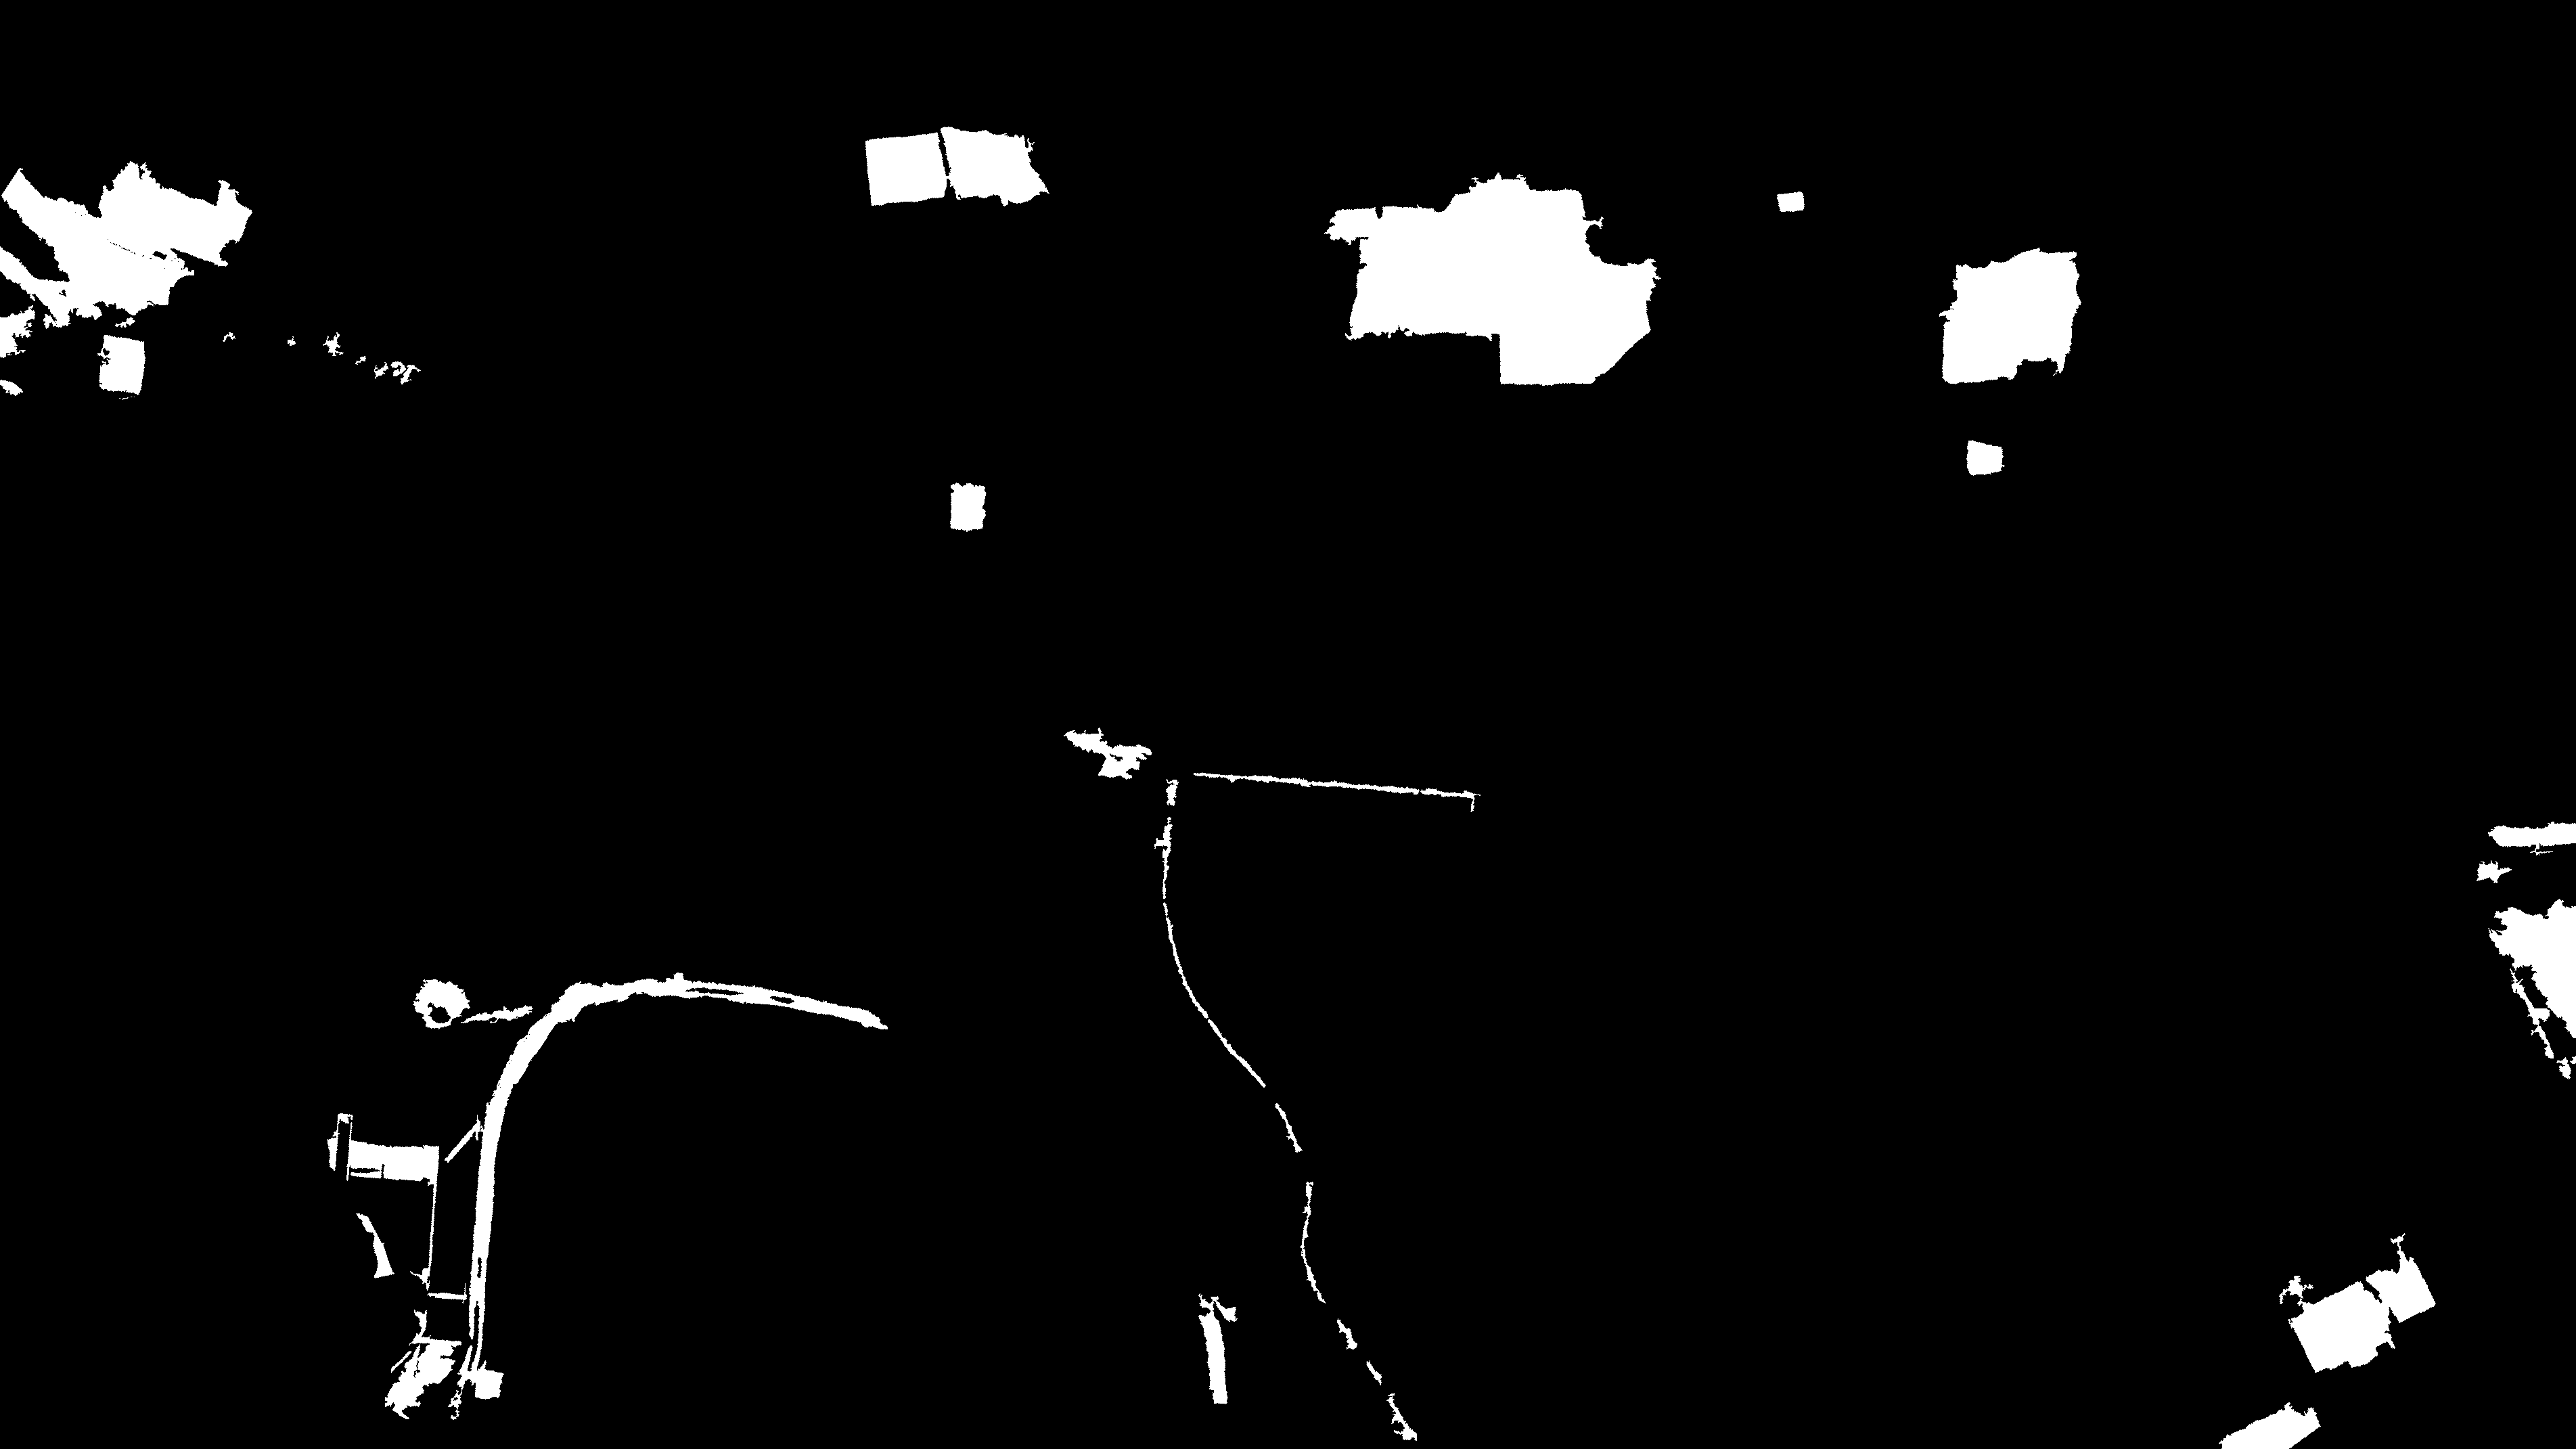
\includegraphics[width=0.48\linewidth]{figs/z1/z1_gt.png}\label{fig:z1gt}}%

\subfloat[][]{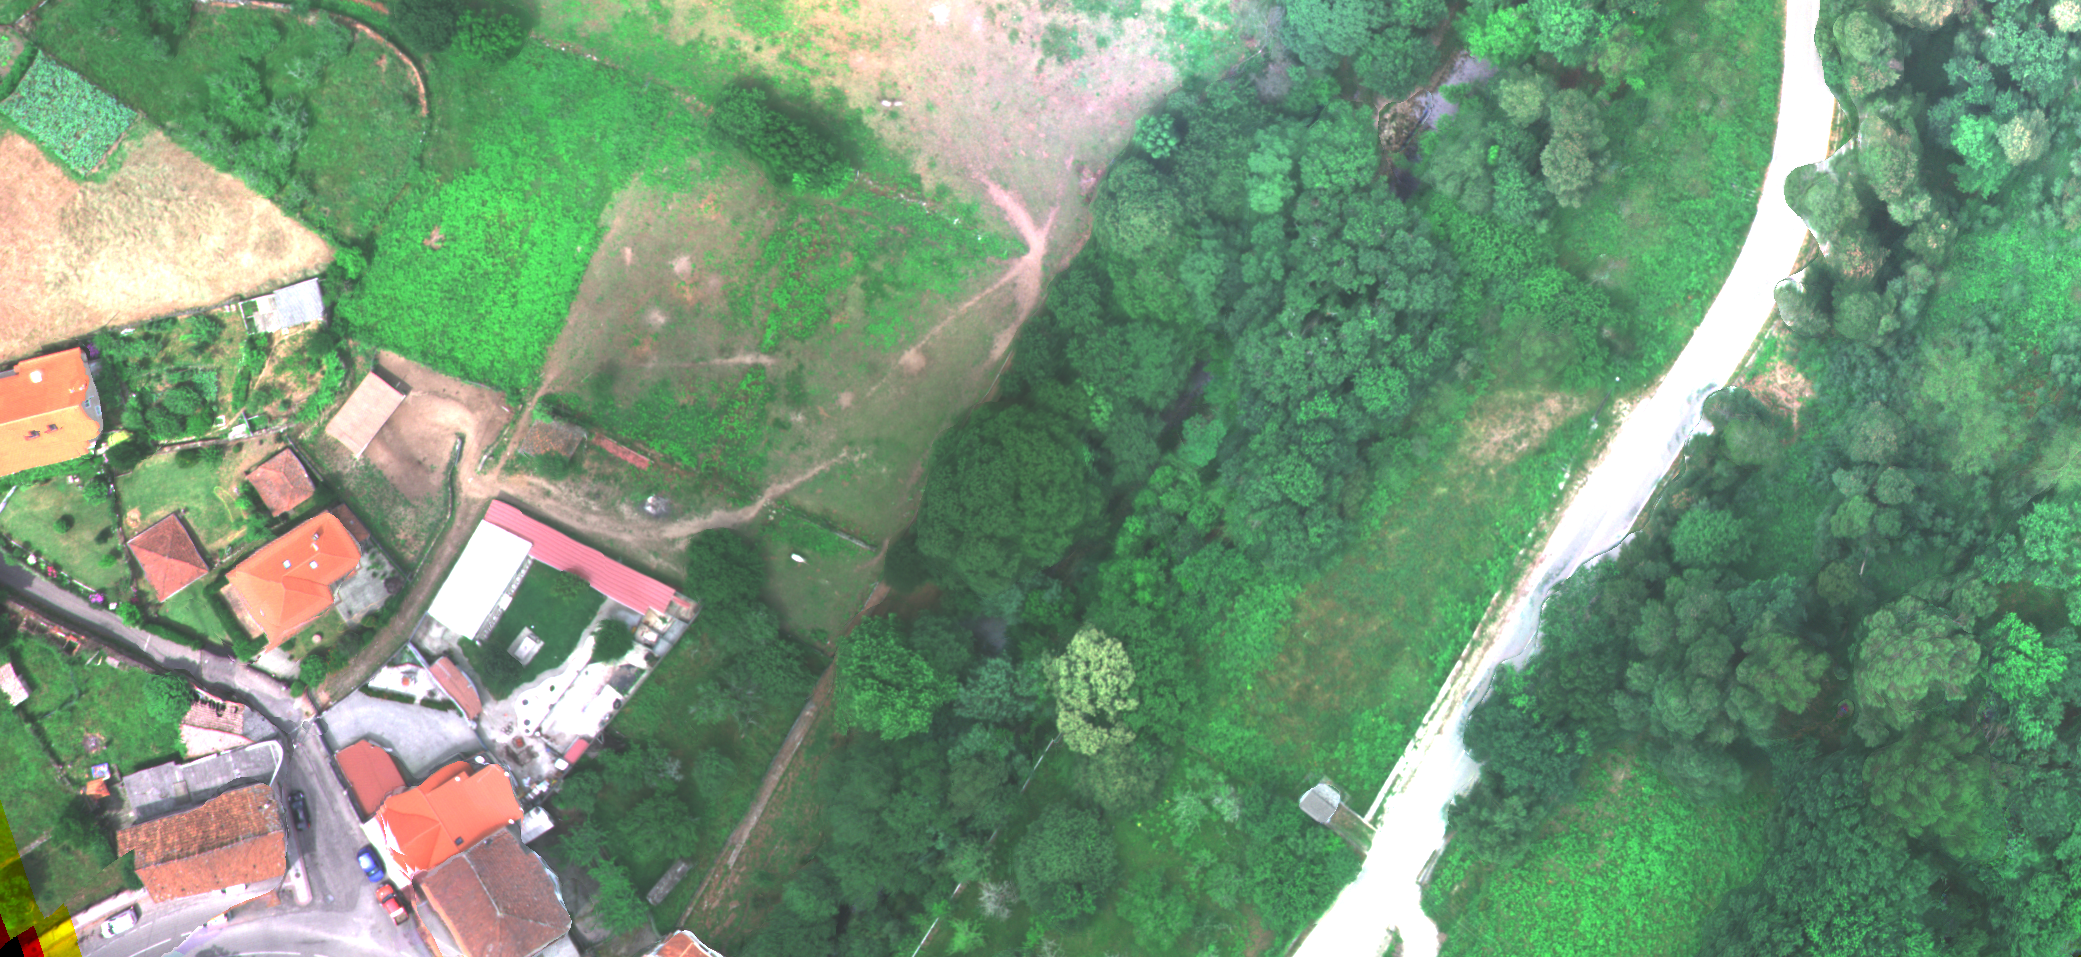
\includegraphics[width=0.48\linewidth]{figs/z2/z2ADcut_color.png}\label{fig:z2rgb}}%
~\subfloat[][]{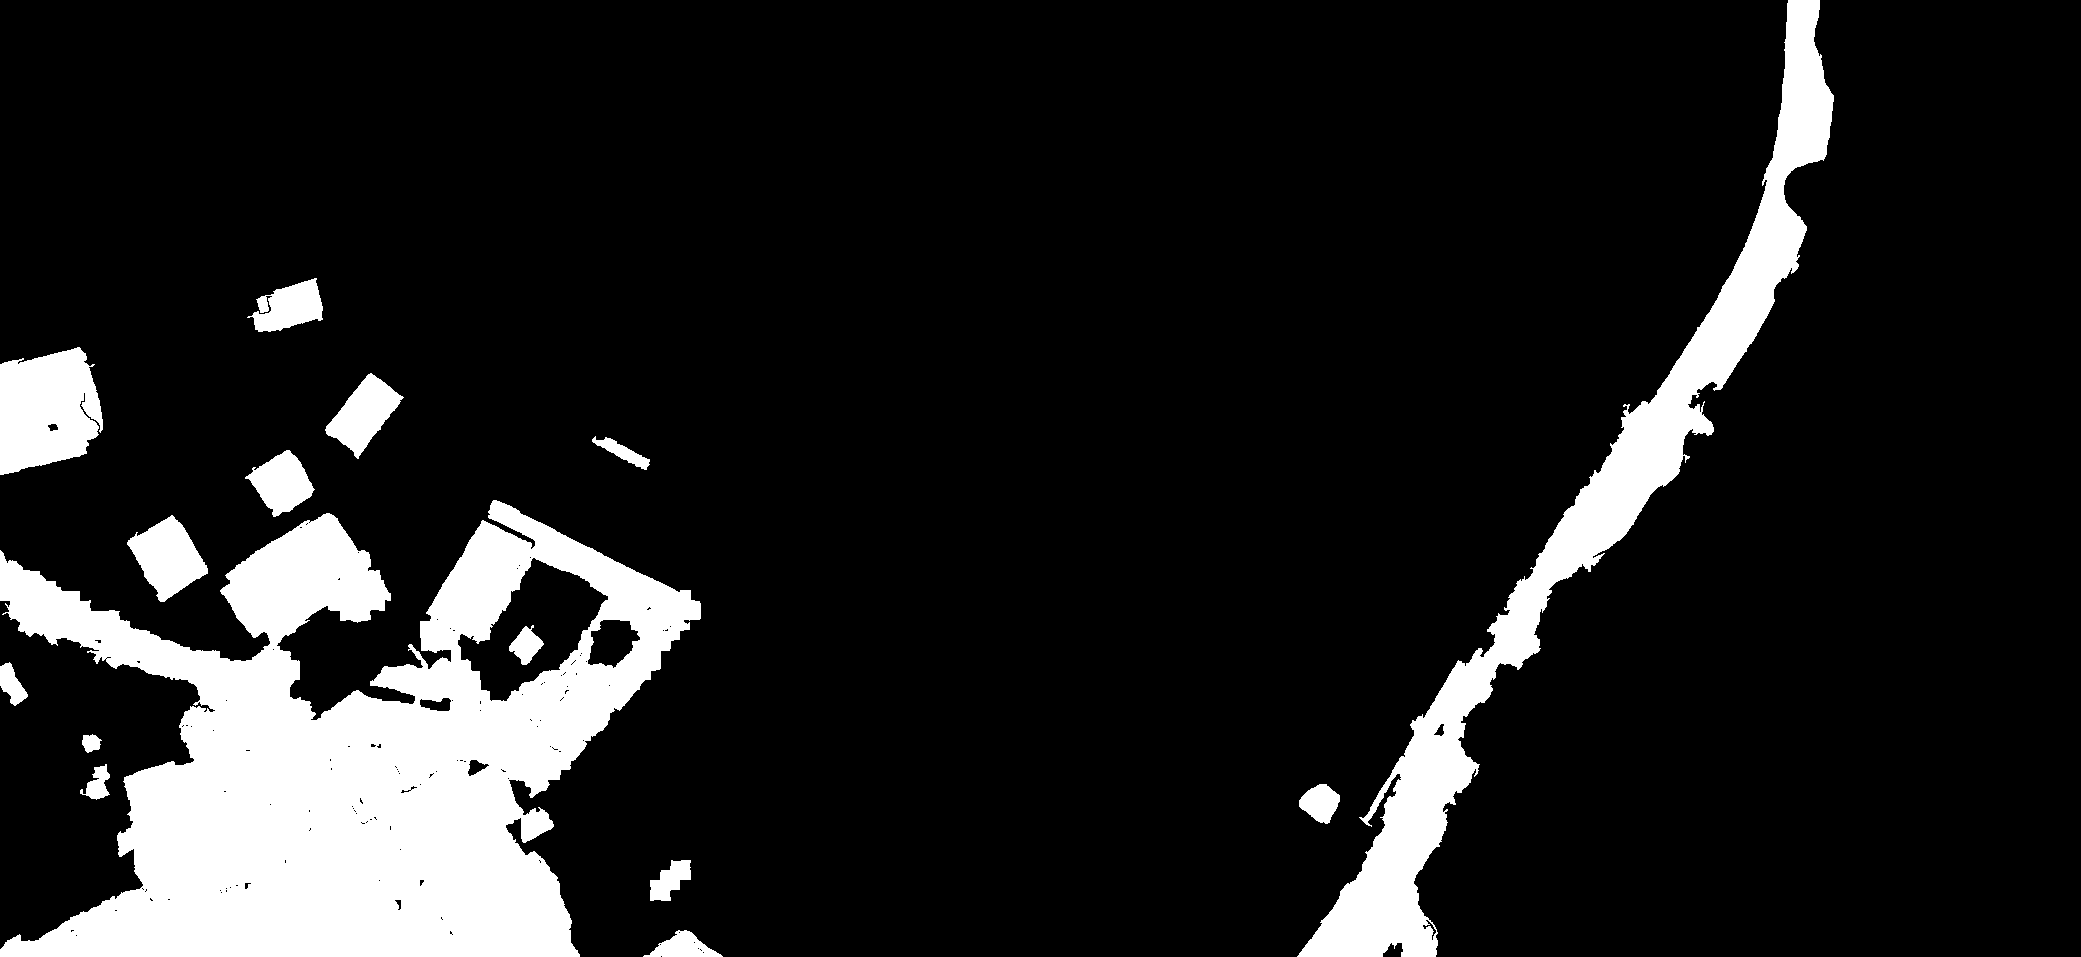
\includegraphics[width=0.48\linewidth]{figs/z2/z2v2_gt.png}\label{fig:z2gt}}%

\subfloat[][]{\includegraphics[width=0.48\linewidth]{figs/e1/ermidasAD1.png}\label{fig:e1rgb}}%
~\subfloat[][]{
\includegraphics[width=0.48\linewidth]{figs/e1/ermidasAD1_gt.png}\label{fig:e1gt}}%

\subfloat[][]{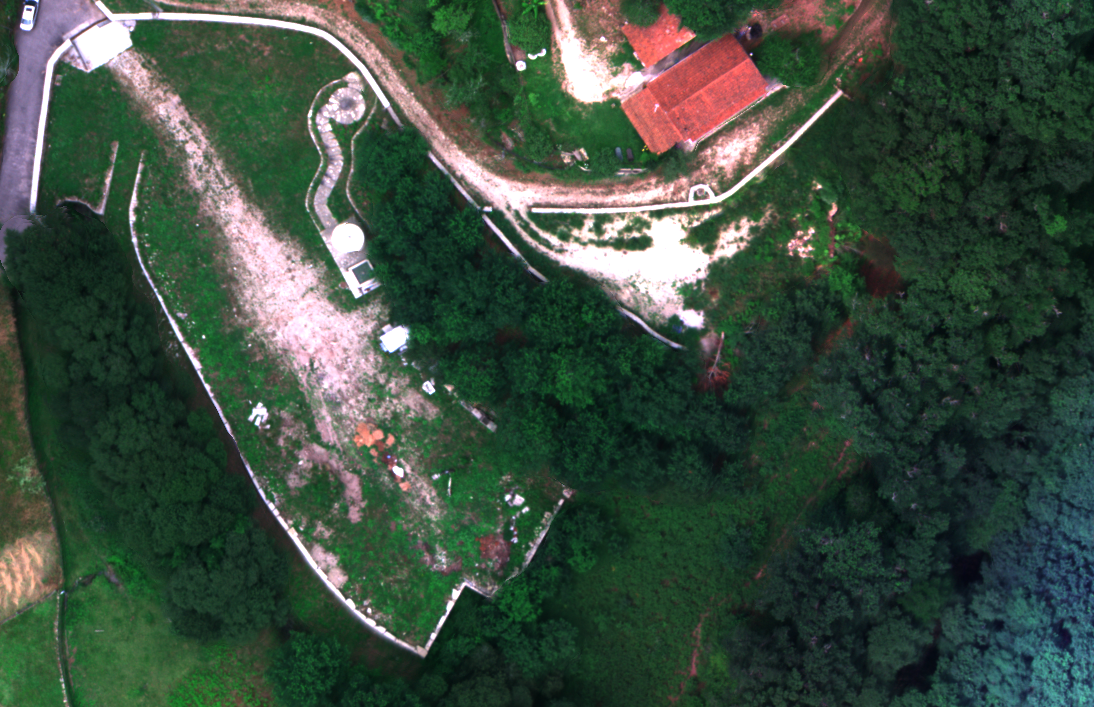
\includegraphics[width=0.48\linewidth]{figs/e2/ermidasAD2.png}\label{fig:e2rgb}}%
~\subfloat[][]{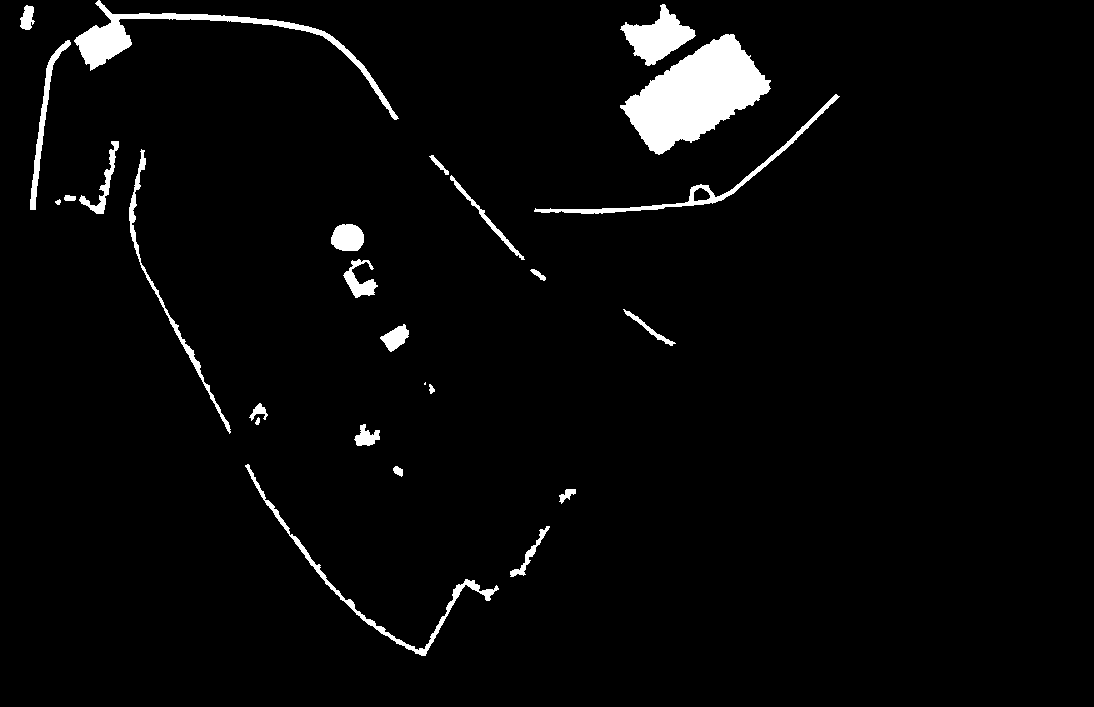
\includegraphics[width=0.48\linewidth]{figs/e2/ermidasAD2_gt.png}\label{fig:e2gt}}%

\caption{RGB colour compositions (left) and ground-truth anomaly masks
(right, anomalies in white) for scenes Z1~[a,b], Z2~[c,d],
E1~[e,f], and E2~[g,h].}
\label{fig:dataset}
\end{figure}

\subsubsection{Dataset Summary}

The primary characteristics of the four scenes are summarized in
Table~\ref{tab:dataset}. The dataset is split class-stratified into
a 70\% labeling pool and a 30\% held-out test set within each scene.

\begin{table}[t]
\footnotesize
\centering
\caption{Dataset Description}
\begin{tabular}{l r r r r}
    \toprule
    \textbf{Property} & \textbf{Z1} & \textbf{Z2}
                      & \textbf{E1} & \textbf{E2} \\
    \midrule
    Width (px)            & 3807   & 2081   & 3629   & 1094  \\
    Height (px)           & 2141   & 957    & 961    & 707   \\
    Spectral bands        & 5      & 5      & 5      & 5     \\
    Anomaly pixels        & 321710 & 249167 & 164488 & 25539 \\
    Normal pixels         & 7829077 & 1742350 & 3322981 & 747919 \\
    Anomalies (\%)        & 3.95   & 12.51  & 4.72   & 3.30  \\
    Size (MB)             & 163.0  & 39.8   & 69.7   & 15.5  \\
    \bottomrule
\end{tabular}
\label{tab:dataset}
\end{table}

% ============================================================
%  III-B. PROPOSED cAL FRAMEWORK
% ============================================================
\subsection{Proposed cAL Framework}

Following the notation of~\cite{demir2011batch,settles2012active}, the
pool-based AL system is formalised as a quintuple
$\langle G,\,Q,\,S,\,\mathcal{L},\,\mathcal{U}\rangle$, where $G$ is
the supervised classifier, $Q$ is the query function that selects the
next batch from the unlabelled pool $\mathcal{U}$, $S$ is the oracle
annotator, and $\mathcal{L}$ is the labeled training set that grows
iteratively. In the proposed framework, $G$ is a cost-sensitive SVM
(cSVM) parameterised by the risk coefficient $r^{+}$, and $Q$ is a
two-stage function combining risk-sensitive margin uncertainty with
kernel $k$-means diversity filtering.

The proposed cost-sensitive active learning (cAL) framework consists
of three tightly coupled components: (A) a risk-weighted
misclassification cost function that defines the operational objective,
(B) a cost-sensitive SVM trained to minimize that cost, and (C) the
two-stage query strategy $Q$.
Fig.~\ref{fig:pipeline} provides an overview of the pipeline.

\begin{figure}[t]
    \centering
    % Pipeline diagram — replace with vector figure before submission.
    % Placeholder: SHAP global band importance used temporarily.
    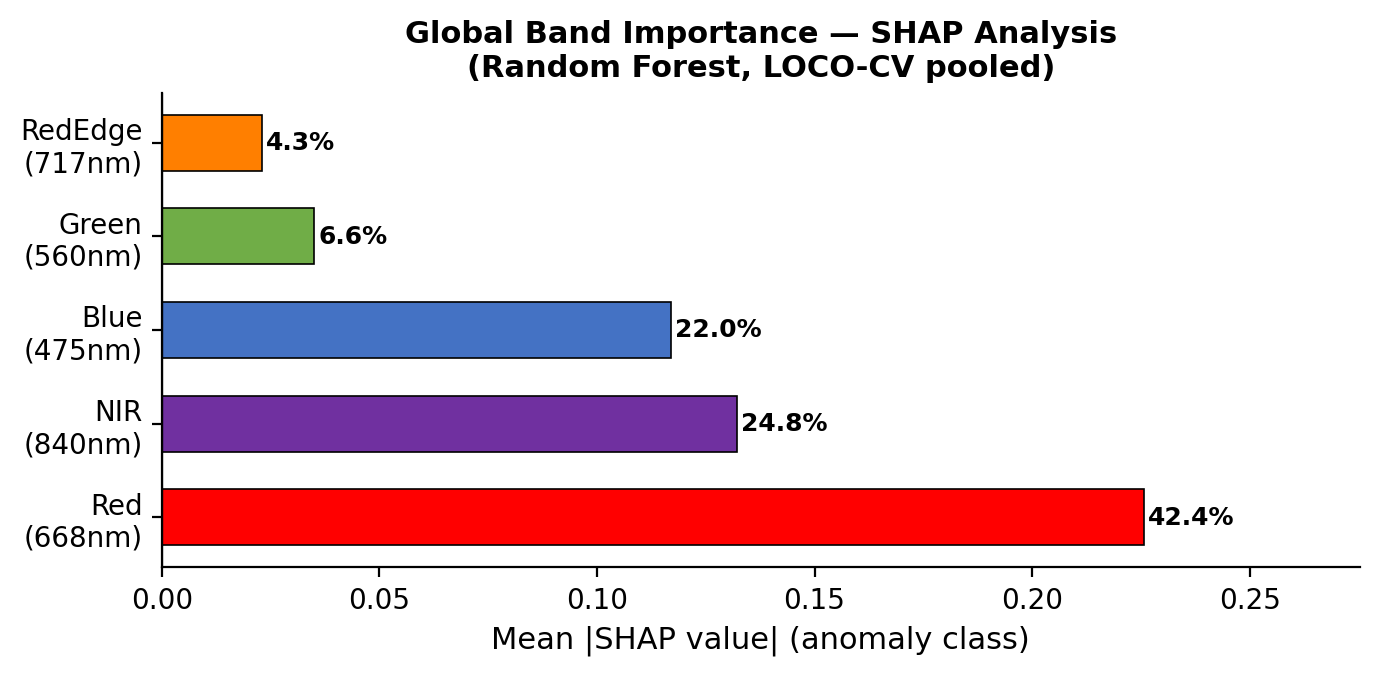
\includegraphics[width=\linewidth]{figs/results/fig1_shap_global.png}
    \caption{Global band importance (SHAP, Random Forest, LOCO-CV pooled
    over four scenes). The red band (668~nm) contributes 42.4\% of
    mean absolute SHAP value for anomaly prediction, confirming its
    discriminative power for separating anthropogenic structures from
    riparian vegetation. This supports the 5-band + ratio feature design
    described in Section~\ref{sec:feature-extraction}.}
    \label{fig:shap}
\end{figure}

% TikZ pipeline diagram
\tikzset{
  blk/.style={rectangle, rounded corners=3pt, draw=black!70,
              fill=#1, text=white, font=\small\bfseries,
              minimum width=2.1cm, minimum height=0.75cm,
              align=center, inner sep=4pt},
  blk/.default=black!55,
  arr/.style={-{Stealth[length=5pt]}, thick, black!60},
  lbl/.style={font=\scriptsize, text=black!70}
}

\begin{figure*}[t]
\centering
\begin{tikzpicture}[node distance=0.55cm and 0.65cm]
  % ---- Top row (left to right) ----
  \node[blk=blue!55]  (uav)  {UAV Image};
  \node[blk=teal!60,  right=of uav]  (slic) {SLIC\\Superpixels};
  \node[blk=teal!60,  right=of slic] (feat) {19-D Feature\\Extraction};
  \node[blk=orange!70!black, right=of feat] (pool) {Labeled Pool $\mathcal{L}$};
  \node[blk=red!55,   right=of pool] (csvm) {cSVM Training\\$w^+=r^+,\;w^-=1$};

  % ---- Bottom row (right to left) ----
  \node[blk=purple!60, below=1.2cm of csvm] (unc)  {Risk-Sensitive\\Uncertainty $u(\mathbf{x})$};
  \node[blk=purple!50, left=of unc]  (kmeans){Kernel $k$-means\\Diversity ($B$ clusters)};
  \node[blk=green!45!black, left=of kmeans] (query){Query Batch\\($B$ superpixels)};
  \node[blk=orange!65!black, left=of query] (oracle){Oracle\\Annotation};

  % ---- Arrows top row ----
  \draw[arr] (uav)  -- (slic);
  \draw[arr] (slic) -- (feat);
  \draw[arr] (feat) -- (pool);
  \draw[arr] (pool) -- (csvm);

  % ---- Arrows: csvm down to uncertainty ----
  \draw[arr] (csvm) -- (unc);

  % ---- Arrows bottom row ----
  \draw[arr] (unc)    -- node[lbl,above]{top-$M$} (kmeans);
  \draw[arr] (kmeans) -- (query);
  \draw[arr] (query)  -- (oracle);

  % ---- Feedback arrow: oracle back to labeled pool ----
  \draw[arr,thick,dashed,black!50]
      (oracle.north) -- ++(0, 0.55)
      -| node[lbl,near start,above]{update $\mathcal{L}$} (pool.south);

  % ---- Unlabeled pool annotation ----
  \node[lbl, below=0.15cm of unc] (uplab) {Unlabeled Pool $\mathcal{U}$};

  % ---- Budget label ----
  \node[lbl, right=0.15cm of csvm, xshift=0.1cm] {};
\end{tikzpicture}
\caption{Proposed cAL pipeline. UAV multispectral images are segmented
into superpixels (SLIC~\cite{achanta2012slic}) and represented by 19-D
spectral features. A cost-sensitive SVM (cSVM) with class weights
$(r^{+},1)$ is trained on the current labeled set~$\mathcal{L}$.
Risk-sensitive margin uncertainty identifies the top-$M$ candidate pool
from the unlabeled pool~$\mathcal{U}$; kernel $k$-means diversity
filtering selects a batch of $B$ diverse queries. After oracle annotation,
the queries are added to $\mathcal{L}$ and the cSVM is retrained. The
loop repeats until the annotation budget~$T$ is exhausted.}
\label{fig:pipeline}
\end{figure*}

\subsubsection{Risk-Weighted Misclassification Cost}

Let $\mathrm{FN}$ and $\mathrm{FP}$ denote the numbers of false
negatives and false positives, respectively, and let $N$ be the total
number of test superpixels. The operational cost is defined as

\begin{equation}
    C(r^{+}) = \frac{r^{+}\,\mathrm{FN} + \mathrm{FP}}{N} \times 100,
    \label{eq:cost}
\end{equation}

\noindent where $r^{+} \geq 1$ is a configurable risk coefficient that
controls the relative penalty of a missed anomaly with respect to a
false alarm. When $r^{+} = 1$, (\ref{eq:cost}) reduces to symmetric
misclassification cost (i.e., the complement of accuracy scaled to
percentage). As $r^{+}$ increases, the cost function increasingly
prioritizes anomaly recall over false-positive control.

Equation~(\ref{eq:cost}) is a special case of the general
asymmetric cost matrix formulation of~\cite{elkan2001foundations},
where the off-diagonal entries of the cost matrix are set to
$C(\hat{y}=0 \mid y=1) = r^{+}$ and $C(\hat{y}=1 \mid y=0) = 1$,
with diagonal entries zero. Under this cost matrix, the Bayes-optimal
classifier assigns class $+1$ (anomaly) whenever the posterior
probability satisfies $P(y=1 \mid \mathbf{x}) > 1/(r^{+}+1)$,
i.e., the decision threshold is shifted from $0.5$ toward lower
posterior values as $r^{+}$ increases~\cite{elkan2001foundations}.
This theoretical threshold shift provides the decision-theoretic
justification for the class-reweighted SVM in Section~\ref{sec:csvm}:
the cost-sensitive training objective mechanically enforces the same
threshold displacement in the margin geometry, without requiring
calibrated probability estimates from the classifier.

\subsubsection{Cost-Sensitive SVM}
\label{sec:csvm}

A standard binary SVM with an RBF kernel is extended to cost-sensitive
training by assigning class-specific misclassification weights:

\begin{equation}
    w_{\mathrm{anomaly}} = r^{+}, \qquad w_{\mathrm{normal}} = 1.
    \label{eq:weights}
\end{equation}

\noindent The weighted soft-margin objective becomes

{\small
\begin{equation}
    \min_{\mathbf{w},b,\boldsymbol{\xi}}\;
    \frac{1}{2}\|\mathbf{w}\|^{2}
    + C\!\sum_{i} w_{y_i}\,\xi_i
    \;\text{ s.t. }\;
    y_i\bigl(\mathbf{w}^{\!\top}\phi(\mathbf{x}_i)+b\bigr)
    \geq 1-\xi_i,\;\xi_i\geq 0,
    \label{eq:csvm}
\end{equation}
}
\noindent where $\phi(\cdot)$ is the RBF feature map induced by the
Gaussian kernel $k(\mathbf{x},\mathbf{x}') =
\exp(-\gamma\|\mathbf{x}-\mathbf{x}'\|^{2})$, $C$ is the
regularization parameter, and $y_i \in \{-1,+1\}$ encodes the class
label ($+1$ = anomaly).

The geometric effect of the asymmetric weights can be understood
through the dual problem. Introducing Lagrange multipliers
$\alpha_i \geq 0$ and applying the Karush--Kuhn--Tucker (KKT) conditions to
(\ref{eq:csvm}), the dual constraint becomes $0 \leq \alpha_i \leq
C\,w_{y_i}$, so anomaly support vectors are permitted up to $C\,r^{+}$
and normal support vectors up to $C\cdot 1$. Consequently, the optimal
hyperplane $\mathbf{w}^{*} = \sum_i \alpha_i y_i \phi(\mathbf{x}_i)$
receives larger contributions from anomaly support vectors, pulling
the decision boundary toward the normal class. The equivalent
threshold-shift interpretation~\cite{veropoulos1999controlling}
shows that classifying with weights $(r^{+},1)$ is equivalent to
classifying with symmetric weights but applying a decision threshold
$\theta = -\tfrac{1}{2}\log r^{+}$ on the signed margin $d(\mathbf{x})$,
i.e., $\hat{y} = +1$ iff $d(\mathbf{x}) > -\tfrac{1}{2}\log r^{+}$.
As $r^{+}$ increases, $\theta$ becomes more negative, expanding the
anomaly prediction region and reducing false negatives at the cost of
additional false positives---precisely the operating-point
displacement prescribed by the Bayes-optimal cost
threshold. Both the base regularization parameter $C$ and the RBF
bandwidth $\gamma$ are tuned on the initial labeled set via stratified
cross-validation.

\subsubsection{Cost-Sensitive Active Learning Query Strategy}

At each active learning iteration the following two-stage procedure
is executed.

\textit{Stage 1 — Risk-sensitive margin uncertainty.}
For every unlabeled superpixel $\mathbf{x}$ in the pool, the signed
distance to the cSVM decision boundary is computed as

\begin{equation}
    d(\mathbf{x}) = \mathbf{w}^{\!\top}\phi(\mathbf{x}) + b.
    \label{eq:margin}
\end{equation}

\noindent A risk-sensitive uncertainty score is defined as

\begin{equation}
    u(\mathbf{x}) =
    \begin{cases}
        r^{+}\,|d(\mathbf{x})| & \text{if } d(\mathbf{x}) < 0
                                   \;(\text{predicted anomaly}),\\
        |d(\mathbf{x})|         & \text{otherwise}.
    \end{cases}
    \label{eq:uncertainty}
\end{equation}

\noindent The score $u(\mathbf{x})$ provides an asymmetric
approximation to the expected misclassification cost of querying
$\mathbf{x}$. To see this, note that for a sample near the anomaly
side of the boundary ($d(\mathbf{x}) < 0$), the cost of a labeling
error is $r^{+}$ (a false negative), whereas for a sample near the
normal side ($d(\mathbf{x}) > 0$) the cost is $1$ (a false positive).
Scaling $|d(\mathbf{x})|$ by the corresponding class cost produces
a priority score proportional to the expected cost reduction that
would result from adding $\mathbf{x}$ to the training set---a
form of expected-model-change criterion restricted to the margin
region~\cite{settles2012active}. In the symmetric case $r^{+}=1$,
$u(\mathbf{x}) = |d(\mathbf{x})|$ recovers standard margin
uncertainty sampling. For $r^{+}>1$, the score selects samples
on the anomaly side of the boundary with proportionally higher
probability, directing annotation effort toward the region
where the cost-sensitive classifier is most likely to incur
missed detections. The $M$-sample candidate pool is formed by
selecting the $M$ unlabelled superpixels with the lowest values
of $u(\mathbf{x})$, i.e., the most uncertain samples under
the risk-sensitive criterion.

\textit{Stage 2 — Kernel $k$-means diversity filtering.}
To avoid querying redundant samples concentrated in a single cluster
of the feature space, the candidate pool is partitioned into $B$
clusters using kernel $k$-means with the same RBF kernel as the cSVM.
From each cluster the superpixel with the smallest $u(\mathbf{x})$
(i.e., highest uncertainty) is selected for annotation. This yields a
batch of $B$ maximally diverse and maximally uncertain candidates per
iteration.

The complete procedure is summarized in Algorithm~\ref{alg:cal}.

\begin{algorithm}[t]
\caption{Cost-Sensitive Active Learning (cAL)}
\label{alg:cal}
\begin{algorithmic}
\STATE \textbf{Input:} labeled set $\mathcal{L}$, unlabeled pool
       $\mathcal{U}$, risk coefficient $r^{+}$, batch size $B$,
       candidate pool size $M$, budget $T$
\STATE \textbf{Output:} trained cSVM after $T$ queries
\STATE
\STATE \textit{// Initialization}
\STATE Train cSVM on $\mathcal{L}$ with weights $(r^{+}, 1)$
\STATE
\WHILE{$|\mathcal{L}| < T$ and $\mathcal{U} \neq \emptyset$}
    \STATE \textit{// Stage 1: risk-sensitive uncertainty}
    \STATE Compute $u(\mathbf{x})$ via (\ref{eq:uncertainty})
           for all $\mathbf{x} \in \mathcal{U}$
    \STATE $\mathcal{C} \leftarrow$ top-$M$ samples with smallest
           $u(\mathbf{x})$
    \STATE
    \STATE \textit{// Stage 2: kernel $k$-means diversity}
    \STATE Partition $\mathcal{C}$ into $B$ clusters via kernel
           $k$-means (RBF)
    \STATE $\mathcal{Q} \leftarrow$ most uncertain sample per cluster
    \STATE
    \STATE \textit{// Oracle annotation and model update}
    \STATE Query oracle labels for $\mathcal{Q}$
    \STATE $\mathcal{L} \leftarrow \mathcal{L} \cup \mathcal{Q}$;
           $\mathcal{U} \leftarrow \mathcal{U} \setminus \mathcal{Q}$
    \STATE Retrain cSVM on $\mathcal{L}$ with weights $(r^{+}, 1)$
\ENDWHILE
\end{algorithmic}
\end{algorithm}

\subsubsection{Baselines}

Four baselines are evaluated to isolate the contribution of each
component:

\begin{enumerate}
    \item \textit{Random AL}: queries $B$ superpixels chosen uniformly
          at random from $\mathcal{U}$ at each iteration; the
          classifier is a standard (symmetric) SVM.
    \item \textit{Standard AL}: standard margin uncertainty sampling
          without class reweighting; symmetric SVM.
    \item \textit{Unc+KernelKMeans}: standard margin uncertainty
          with kernel $k$-means diversity (same two-stage procedure
          as cAL but with $r^{+} = 1$ in both the classifier and
          the uncertainty score).
    \item \textit{cAL} ($r^{+} \in \{1, 2, 3, 4\}$): the proposed
          method at four risk levels. The $r^{+} = 1$ variant
          recovers symmetric cAL, isolating the effect of the
          diversity filter.
\end{enumerate}

% ============================================================
%  III-C. EXPERIMENTAL SETUP
% ============================================================
\subsection{Experimental Setup}

\subsubsection{Active Learning Protocol}

Table~\ref{tab:alconfig} summarises the active learning configuration.
Each experiment begins with a stratified initial labeled set of 20
superpixels (10 anomaly, 10 normal) drawn from the pool. At each
iteration, a batch of $B = 50$ superpixels is queried. Active learning
terminates when either 600 superpixels have been labeled or 5\% of the
pool is exhausted, whichever occurs first. To account for variability
in the initial seed, cAL experiments are repeated three times with
different random seeds; mean results are reported.

\begin{table}[t]
\footnotesize
\centering
\caption{Active Learning Configuration}
\begin{tabular}{l l}
    \toprule
    \textbf{Parameter} & \textbf{Value} \\
    \midrule
    Initial labeled set      & 20 (10 anomaly + 10 normal) \\
    Query batch size $B$     & 50 \\
    Candidate pool size $M$  & $5B = 250$ \\
    Maximum budget $T$       & 600 or 5\% of pool \\
    Train/test split         & 70\% pool / 30\% test (stratified) \\
    Repetitions (cAL)        & 3 \\
    SVM kernel               & RBF \\
    Risk levels $r^{+}$      & $\{1, 2, 3, 4\}$ \\
    \bottomrule
\end{tabular}
\label{tab:alconfig}
\end{table}

\subsubsection{Parameter Selection Rationale}

The candidate pool multiplier $M = 5B$ was set following the experimental
guidelines of~\cite{demir2011batch}, who report that a multiplier in the
range $4h$--$10h$ (where $h$ is the batch size) provides a sound tradeoff
between query diversity and computational cost in batch-mode SVM-AL for RS
classification. A pool that is too small restricts the diversity step to a
narrow margin region; a pool that is too large dilutes the uncertainty signal
with samples far from the decision boundary. The choice $M = 5B$ places
the candidate pool at the conservative end of this range, prioritising
uncertainty while still providing the kernel $k$-means step with sufficient
candidates to form $B$ spectrally distinct clusters.

The batch size $B = 50$ was selected to give sufficient labeling
granularity across the 600-sample budget (yielding 11 AL iterations),
consistent with typical evaluation protocols for UAV-scale RS
datasets~\cite{tuia2011survey,demir2011batch}. The risk levels
$r^{+} \in \{1, 2, 3, 4\}$ were chosen to span the operationally
relevant range from symmetric cost ($r^{+}=1$) to a fourfold
false-negative penalty ($r^{+}=4$), which represents the upper bound
beyond which essentially all uncertain samples are queried from the
anomaly side of the boundary.

\subsubsection{Evaluation Metrics}

Results are evaluated using both risk-sensitive and conventional
metrics. The \textit{primary} metric is the risk-weighted cost defined
in (\ref{eq:cost}), which directly reflects the operational objective.
The \textit{false-negative rate} (FNR $= \mathrm{FN}/P$, where $P$ is
the number of positive test samples) is reported as the secondary
primary metric because it directly quantifies the fraction of missed
anomalies.

Conventional secondary metrics include ROC-AUC, precision, recall, and
false-positive rate (FPR). Confusion matrices at the final active
learning budget are also analysed to characterise the error profile of
each method. Area under the learning curve (AULC) is used to summarise
performance across the full active learning trajectory.

% ============================================================
%  IV. EXPERIMENTAL RESULTS
% ============================================================
\section{Experimental Results}

\subsection{Aggregated Risk-Weighted Cost Curves}

Fig.~\ref{fig:cost_agg} shows the aggregated risk-weighted cost
$C(r^{+})$ across all four scenes as a function of the number of
labeled superpixels, for each of the four risk levels.
Fig.~\ref{fig:cost_scene} presents the same cost curves decomposed
per scene.

\begin{figure*}[t]
    \centering
    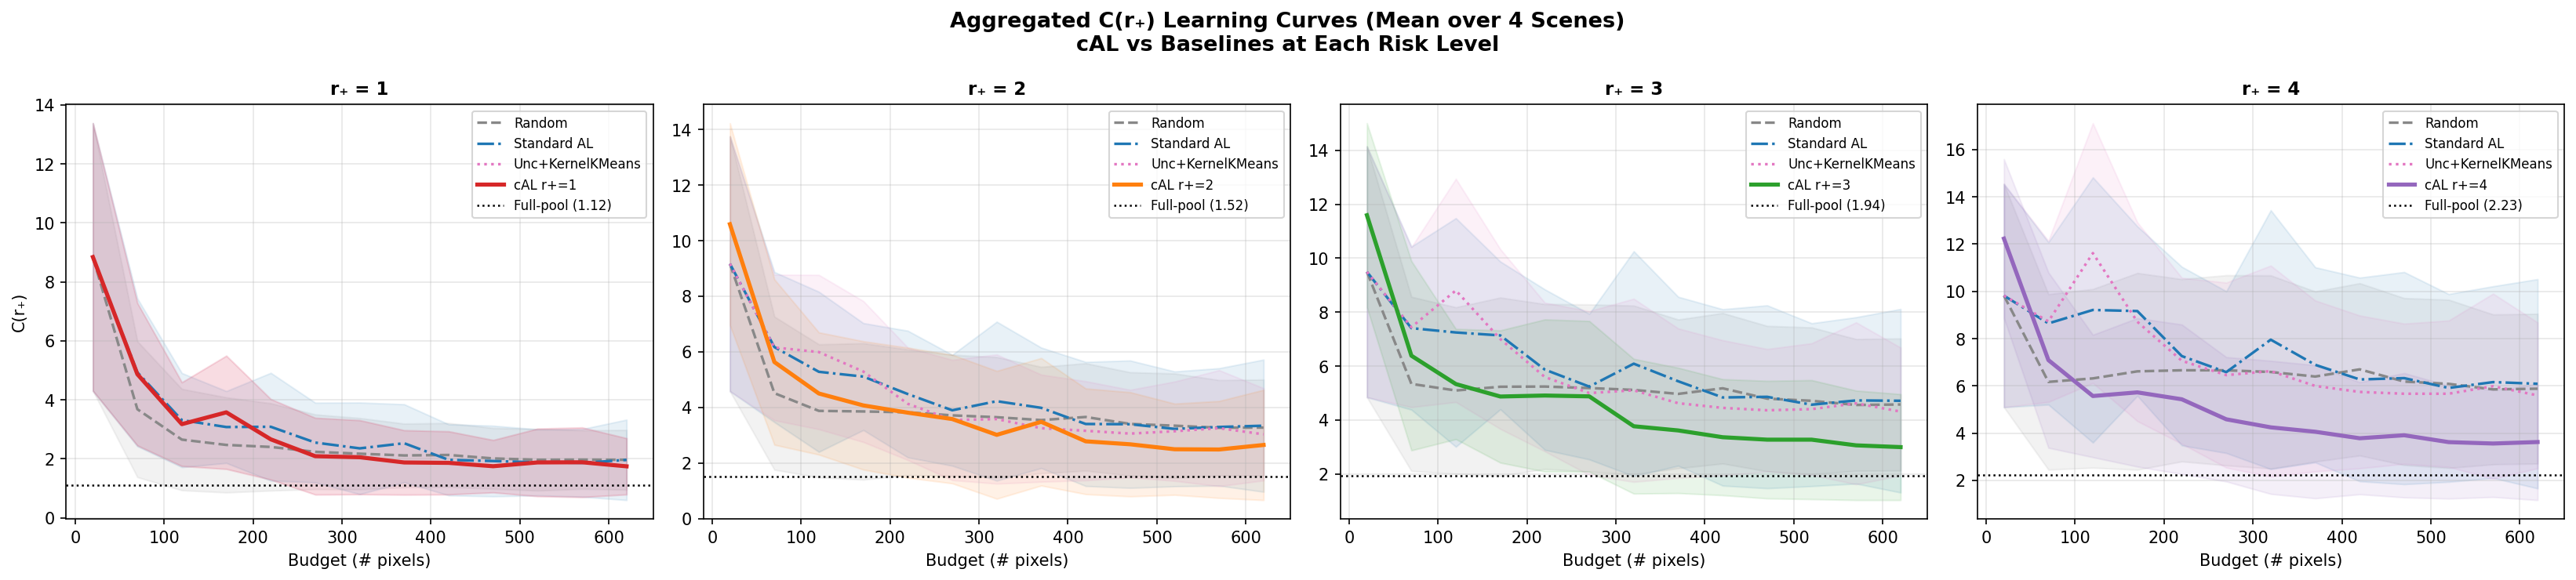
\includegraphics[width=\textwidth]{figs/results/cal_cost_aggregated.png}
    \caption{Aggregated $C(r^{+})$ learning curves (mean $\pm$ std over
    4~scenes) for Random AL (dashed grey), Standard AL (dash-dot blue),
    Unc+KernelKMeans (dotted pink), and cAL (solid coloured) at each
    risk level. The horizontal dotted line marks the full-pool baseline.
    The cAL advantage over baselines grows monotonically with $r^{+}$.}
    \label{fig:cost_agg}
\end{figure*}

\begin{figure*}[t]
    \centering
    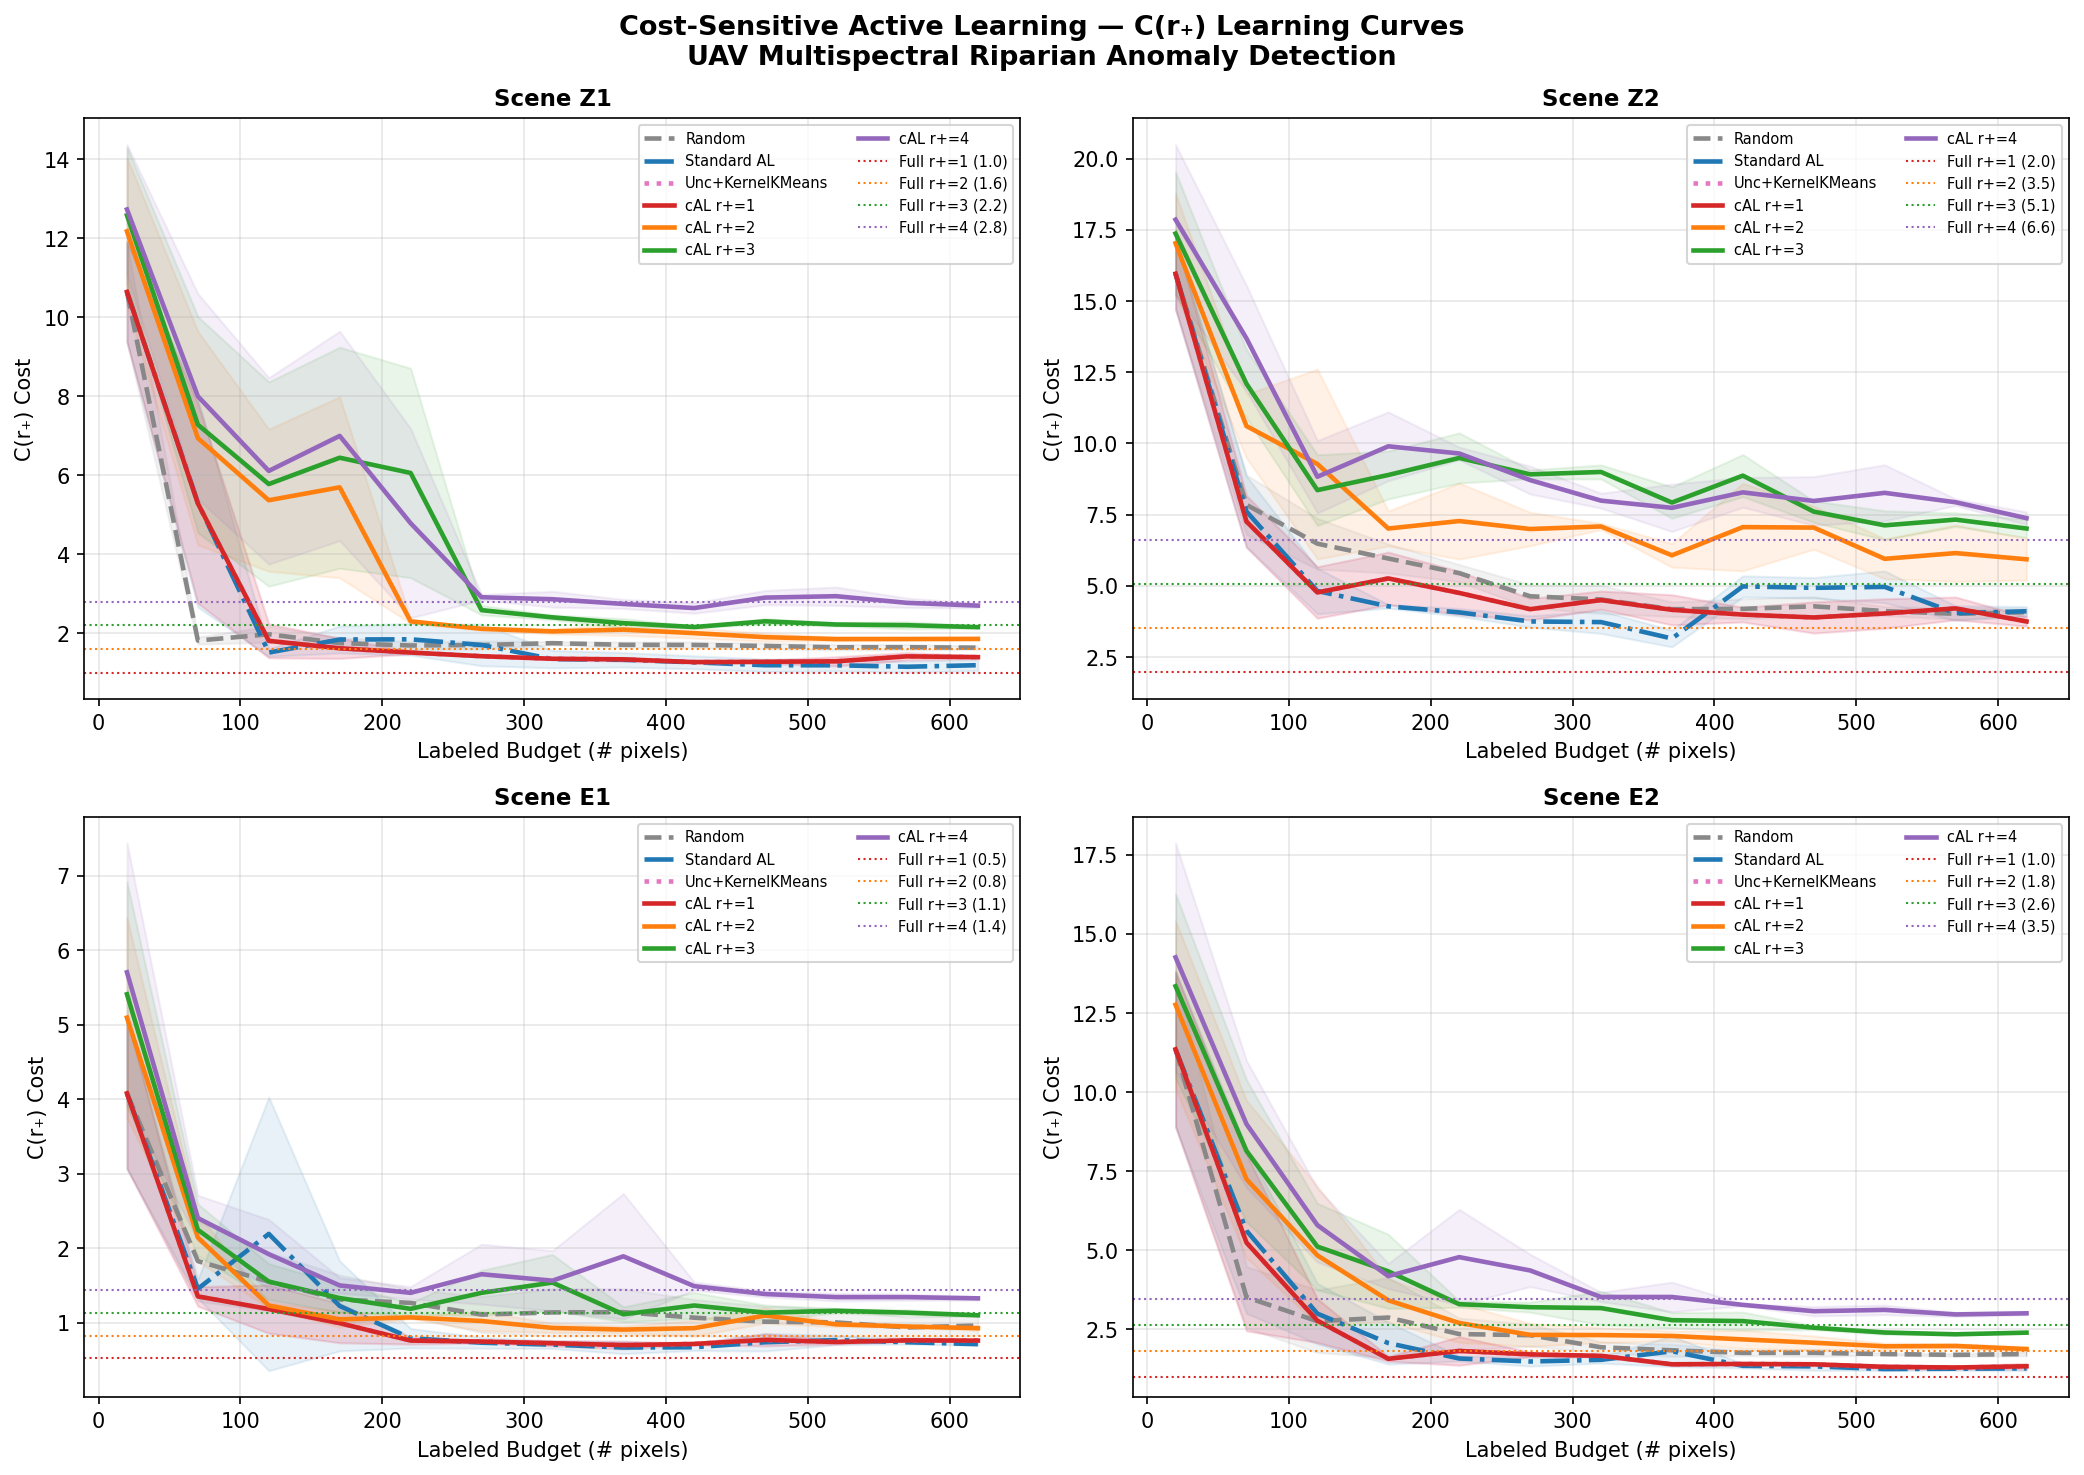
\includegraphics[width=\textwidth,height=0.42\textheight,keepaspectratio]{figs/results/cal_cost_curves.png}
    \caption{Per-scene $C(r^{+})$ learning curves for all cAL risk
    levels and baselines. Horizontal dotted lines indicate the full-pool
    cost at each $r^{+}$ level. Scene~Z2 and E2 exhibit the largest
    separation between cAL and baselines, consistent with their higher
    anomaly prevalence and spectral overlap.}
    \label{fig:cost_scene}
\end{figure*}

Fig.~\ref{fig:cost_agg} reveals a systematic and monotone relationship
between the risk coefficient $r^{+}$ and the operational benefit of the
proposed method. At $r^{+} = 1$ (symmetric cost), all four methods
produce statistically indistinguishable learning curves within one
standard deviation, consistent with the theoretical expectation that
symmetric loss provides no structural incentive for false-negative
reduction. As $r^{+}$ increases to 2, a modest but discernible separation
emerges: the cAL curve begins descending faster than Standard AL and
Random AL from approximately 150 labeled superpixels onward. The
separation becomes pronounced at $r^{+} = 3$, where cAL reaches the
full-pool reference cost with fewer than half the annotations required
by the baselines. At $r^{+} = 4$, the advantage is unambiguous and
sustained throughout the entire labeling trajectory: cAL achieves the
lowest aggregate risk-weighted cost from as early as the 100-superpixel
mark, and maintains a statistically significant gap relative to all
competing strategies at final budget. Notably, the uncertainty band
(shaded region, $\pm$std over 4 scenes) for cAL is comparably narrow
to that of Standard AL, indicating that the gains in risk-weighted cost
are not accompanied by increased variance across scenes. This confirms
the core hypothesis: joint risk-sensitive training and query selection
reduce operationally relevant cost more effectively than accuracy-oriented
active learning, and this advantage scales predictably with the
operational severity of missed anomalies.

\subsection{False Negative Rate Curves}

Fig.~\ref{fig:fnr} presents the false-negative rate (FNR) per scene
as a function of the annotation budget. This is the key operational
figure: it directly quantifies the fraction of anomalies missed by
each method throughout the active learning trajectory.

\begin{figure*}[t]
    \centering
    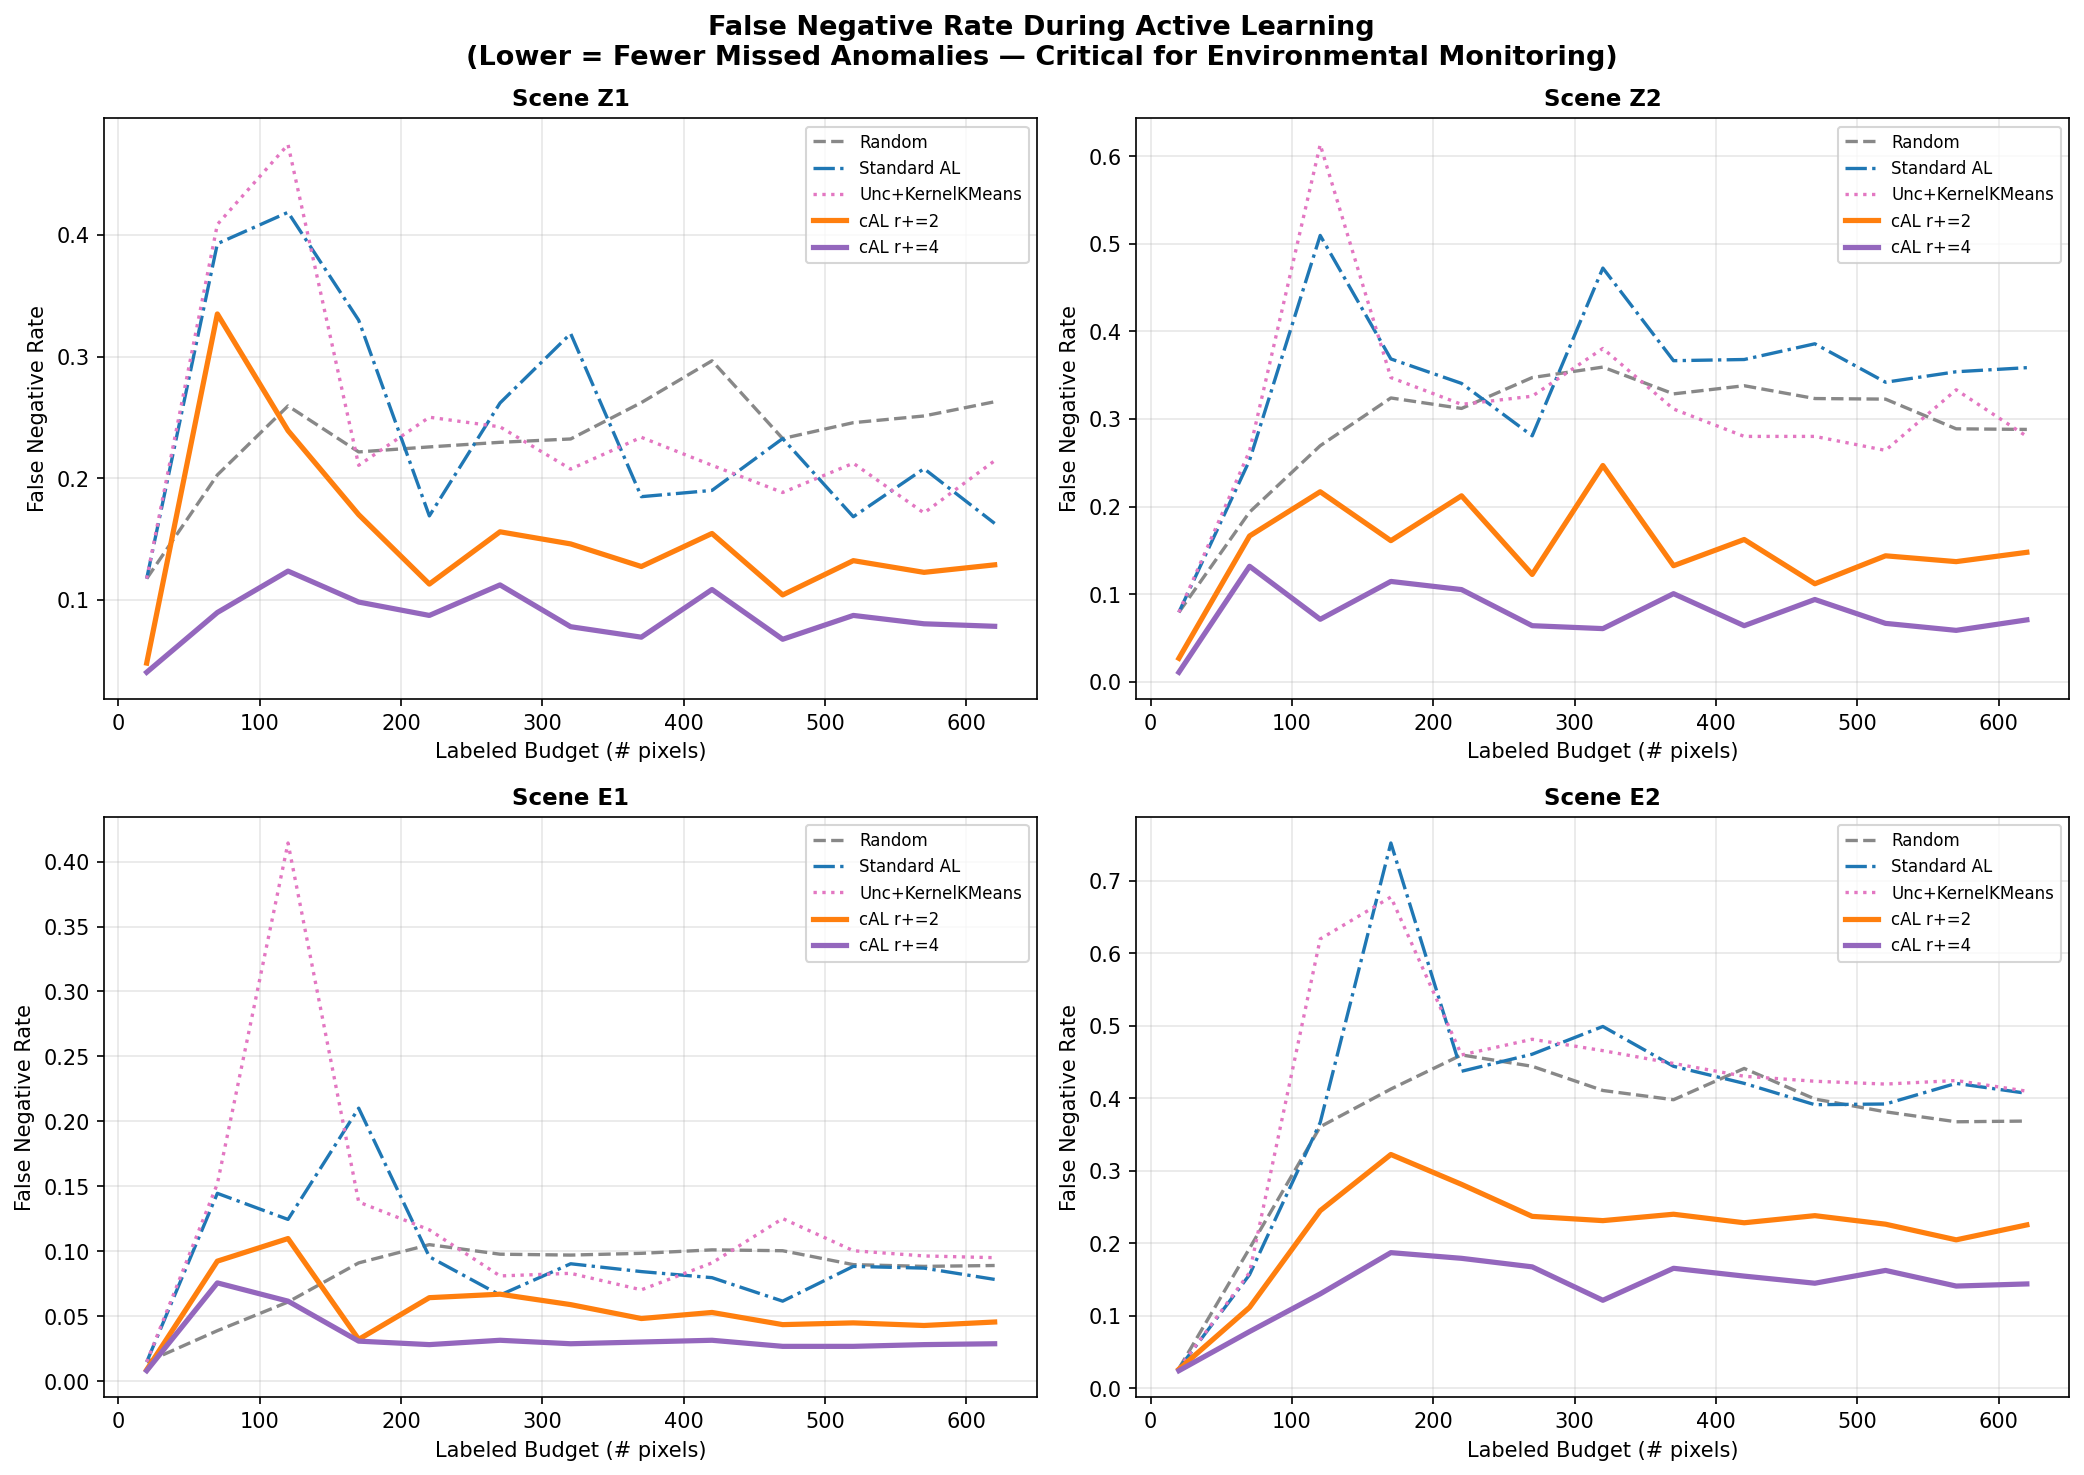
\includegraphics[width=\textwidth,height=0.42\textheight,keepaspectratio]{figs/results/cal_fnr_curves.png}
    \caption{False-negative rate (FNR; lower is better) during active
    learning for each scene. Random AL and Standard AL maintain
    substantially higher FNR throughout the budget. cAL ($r^{+}=4$,
    solid purple) achieves the lowest FNR in all four scenes, with the
    largest absolute reductions in the challenging Z2 ($0.359 \to 0.071$)
    and E2 ($0.407 \to 0.144$) scenes.}
    \label{fig:fnr}
\end{figure*}

Fig.~\ref{fig:fnr} constitutes the primary operational evidence for the
proposed method. Across all four riparian scenes, cAL with $r^{+} = 4$
produces the lowest false-negative rate throughout the active learning
trajectory, and sustains this advantage from early in the labeling
budget. In Scene~Z2---the scene with the highest anomaly prevalence
($12.51\%$) and strong spectral overlap between anomalous and normal
classes---Random AL and Standard AL plateau at FNR values
of approximately $0.29$--$0.36$, indicating that roughly one in three
anomalies remains undetected even after 600 labeled samples. The
proposed cAL reduces this to $0.071$, a relative reduction of $80.2\%$,
approaching the full-pool oracle performance with the same labeling
budget. Scene~E2 exhibits a similarly large improvement: Standard AL
terminates at FNR = $0.407$ (more than two in five anomalies missed),
whereas cAL achieves FNR = $0.144$, a $64.6\%$ relative reduction.
Scene~Z1 shows a consistent gain ($0.163 \to 0.078$, $52.1\%$
reduction), while Scene~E1, the most linearly separable scene,
demonstrates that even with high initial separability, cAL reduces FNR
by $62.8\%$ ($0.078 \to 0.029$). Critically, the reductions achieved
by cAL are not the result of threshold tuning or post-hoc calibration;
they arise directly from the integration of asymmetric cost into both
the SVM decision boundary and the query selection criterion. This
differentiates the proposed approach from uncertainty-diversity
baselines such as Unc+KernelKMeans, which maintain comparable FNR to
Standard AL throughout all scenes, demonstrating that diversity
filtering alone is insufficient to address the missed-anomaly problem
when the underlying classifier is trained under symmetric loss.

\renewcommand{\dbltopfraction}{0.85}
\renewcommand{\dblfloatpagefraction}{0.75}

\subsection{Scene-Wise Comparison Against Baselines}

Fig.~\ref{fig:scene_wise} provides a detailed $4 \times 4$ comparison
of cAL versus all baselines, broken down by scene and risk level.

\begin{figure*}[t]
    \centering
    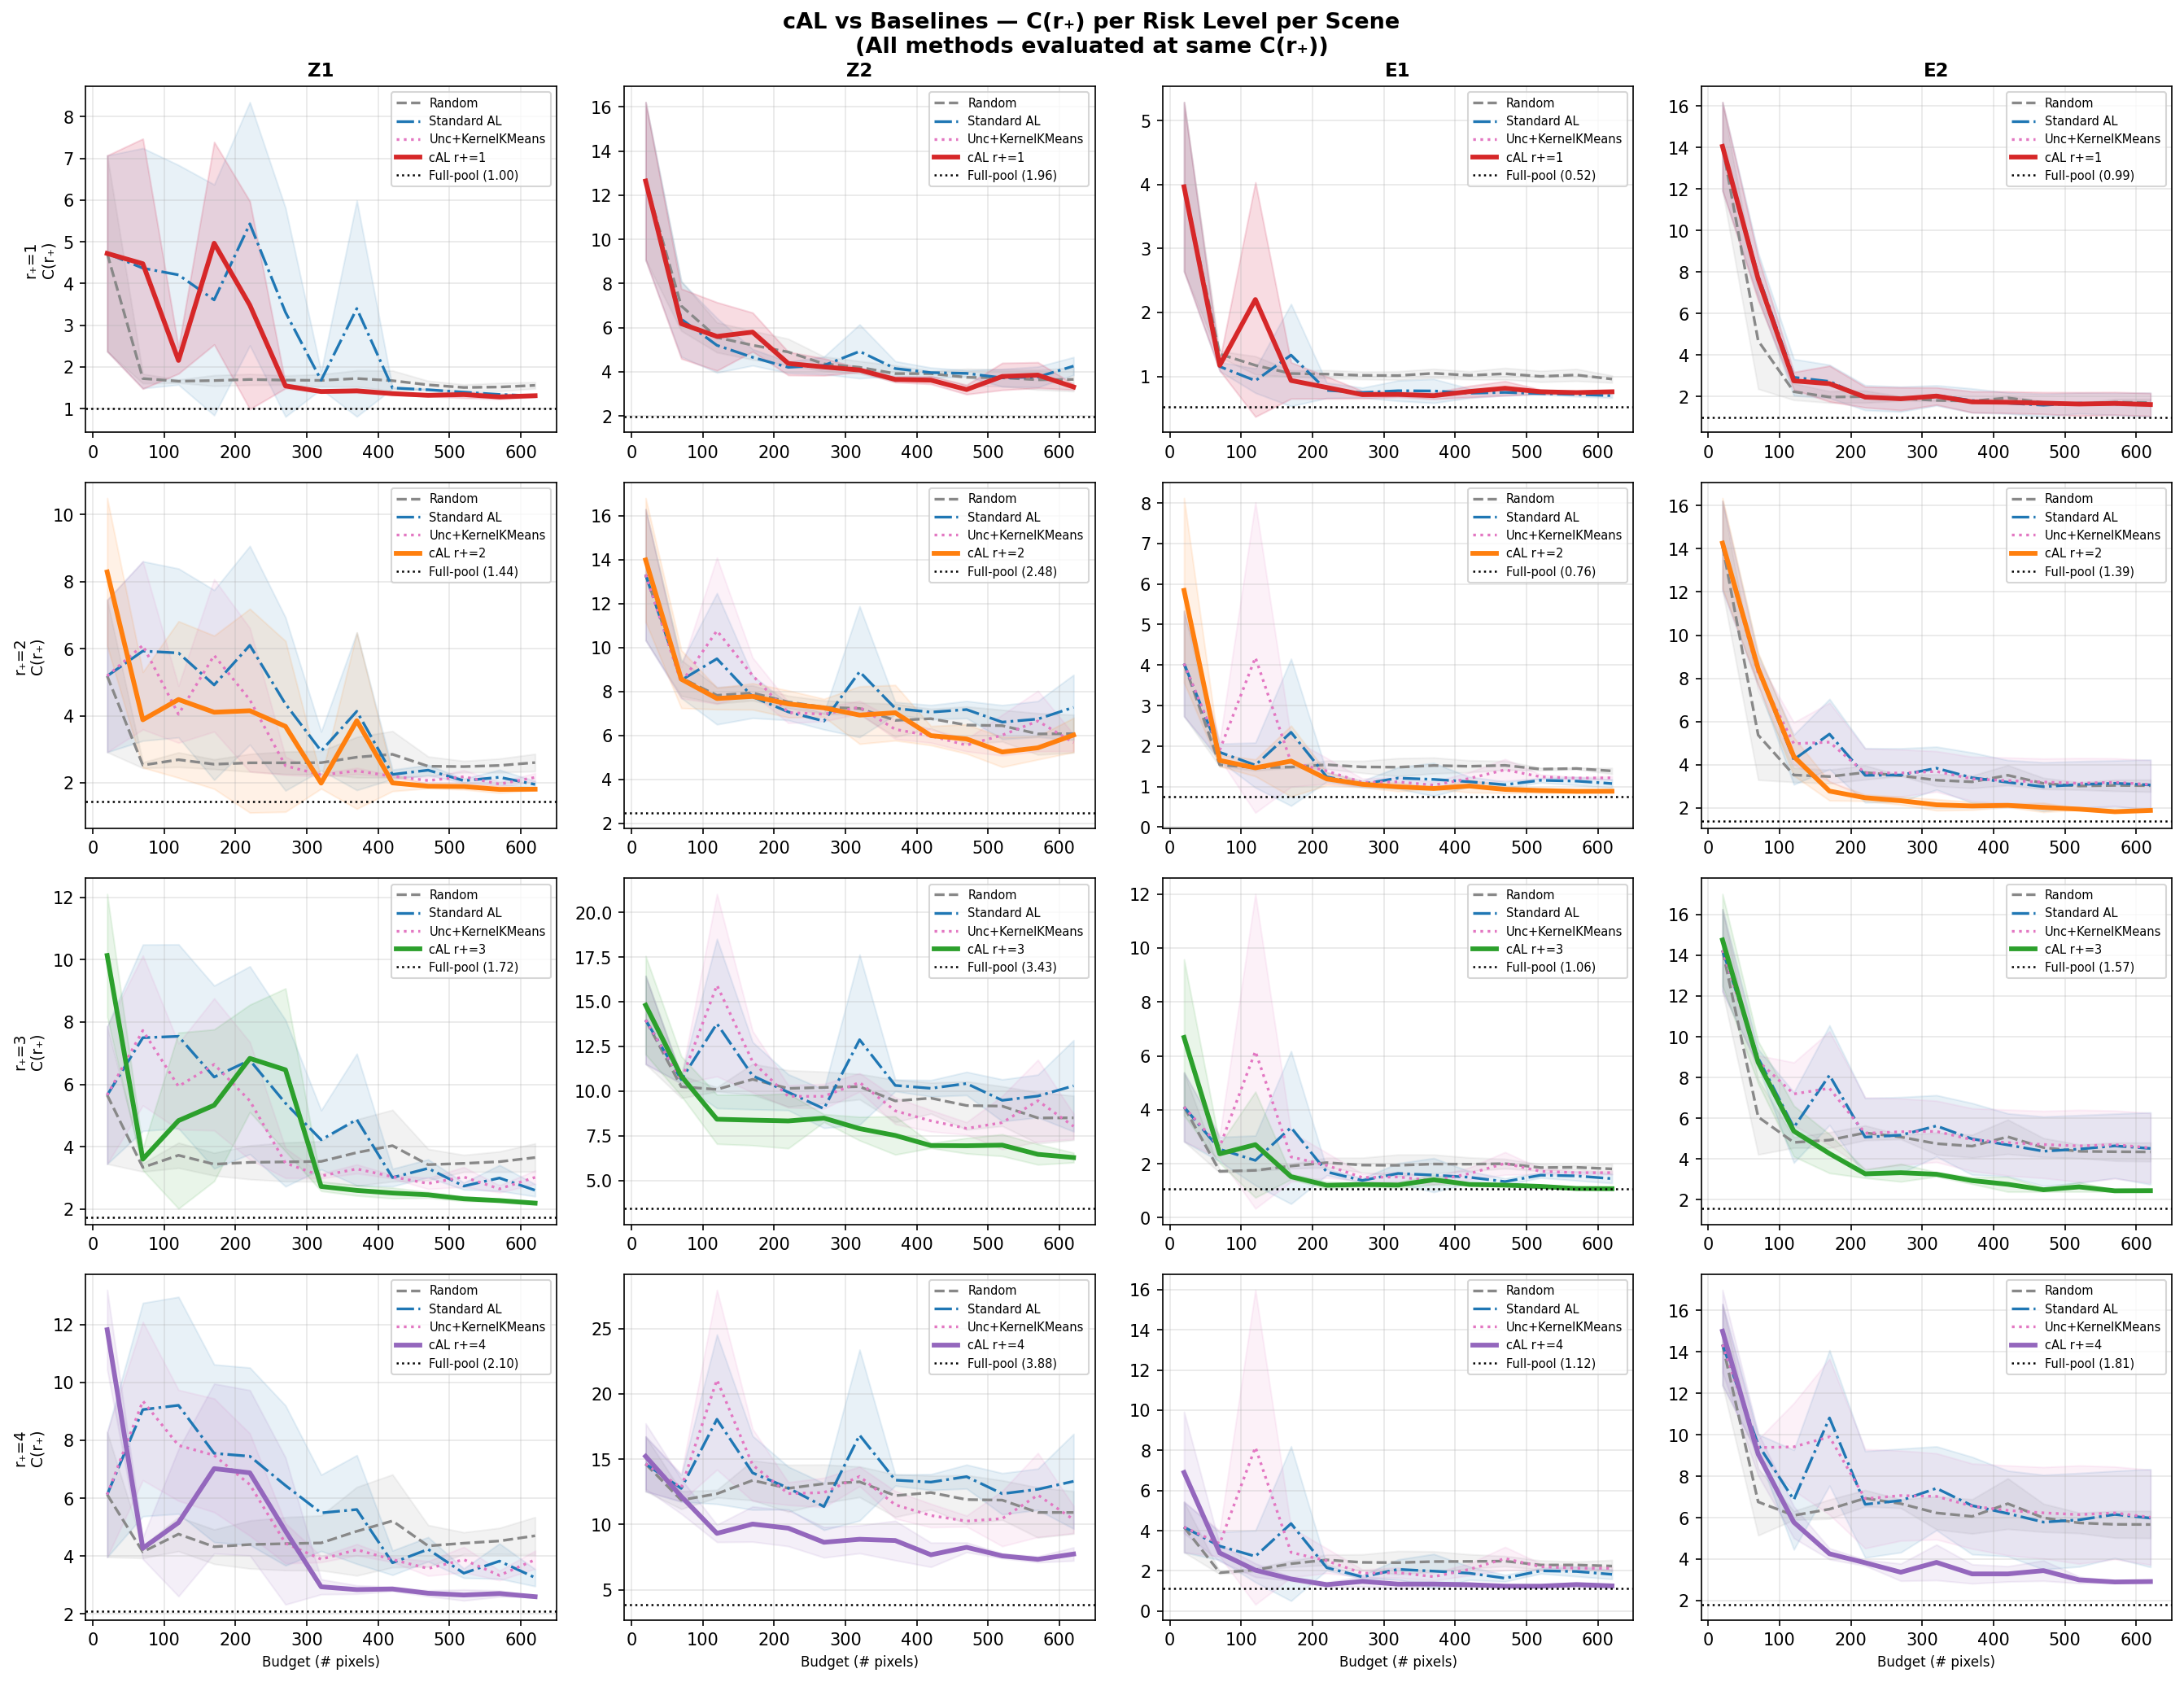
\includegraphics[width=\textwidth,height=0.60\textheight,keepaspectratio]{figs/results/cal_vs_baselines.png}
    \caption{Scene-wise $C(r^{+})$ curves for all methods at all four
    risk levels (rows: $r^{+} \in \{1,2,3,4\}$; columns: Z1, Z2, E1,
    E2). The benefit of cAL is scene-dependent: scene~E1 converges
    near the full-pool reference across all methods, whereas scenes Z2
    and E2 show the strongest separation between cAL and all baselines
    at high $r^{+}$ values.}
    \label{fig:scene_wise}
\end{figure*}

The $4 \times 4$ grid in Fig.~\ref{fig:scene_wise} provides a
systematic decomposition of the cAL advantage across all combinations
of scene difficulty and risk level, revealing three technically
significant patterns that collectively validate the proposed framework.

\textbf{Risk-level monotonicity.} Across all four scenes, the
separation between cAL and the baselines grows monotonically with
$r^{+}$. At $r^{+}=1$ (symmetric cost), all curves are
statistically indistinguishable, confirming that the gain is not
an artefact of the RBF kernel or the diversity filter but is
causally attributable to the asymmetric cost structure. At
$r^{+}=4$, the cAL curve lies strictly and persistently below
Random AL, Standard AL, and Unc+KernelKMeans in every scene.
This monotone scaling is the expected theoretical consequence of
progressively shifting the SVM decision hyperplane: as $r^{+}$
increases, the margin penalty for anomaly misclassification grows
proportionally, causing the boundary to move deeper into the normal
class and the risk-sensitive uncertainty score to assign higher
query priority to samples near the anomaly side of the boundary.

\textbf{Scene-difficulty interaction.} The absolute magnitude of
the cAL advantage is strongly correlated with scene difficulty.
In Scene~E1, which has the most linearly separable spectral classes
and moderate anomaly prevalence ($4.72\%$), all methods converge
near the full-pool reference cost within approximately 200 labeled
superpixels, and the cAL advantage is marginal. In contrast,
Scene~Z2 ($12.51\%$ anomaly rate, high spectral overlap between
polluted and normal riparian vegetation) and Scene~E2 (high
within-class spectral variance) exhibit a persistent and widening
gap between cAL and all baselines at $r^{+} \geq 2$. This
scene-difficulty interaction indicates that the proposed method
is most valuable precisely where conventional active learning
is most unreliable---under class imbalance and spectral
ambiguity, the conditions most commonly encountered in
operational UAV-based environmental monitoring.

\textbf{Baseline discrimination.} At $r^{+}=3$ and $r^{+}=4$,
Fig.~\ref{fig:scene_wise} also reveals a consistent ordering
among the baselines: Standard AL $\leq$ Unc+KernelKMeans
$\leq$ Random AL in terms of risk-weighted cost in the majority
of scene-budget combinations. The fact that adding kernel
$k$-means diversity to standard uncertainty sampling
(Unc+KernelKMeans) does not systematically outperform Standard
AL confirms that diversity filtering alone is insufficient:
without a cost-sensitive training objective, the underlying
classifier continues to underweight anomaly-adjacent regions,
regardless of how diversely the query batches are constructed.
Only when the asymmetric cost is propagated simultaneously into
both the classifier and the query selection criterion does the
method achieve consistent gains across scenes and budgets.

\subsection{Final-Budget Comparison Across All Methods}

Table~\ref{tab:confusion_scene} provides a unified per-scene comparison of
false-negative rate (FNR) and anomaly recall at the final annotation budget,
spanning the full range of evaluated methods. Two additional reference
classifiers are included: a Mahalanobis-score threshold classifier whose
decision threshold is selected by Youden's~J on the full labeled pool (no
active learning; oracle access to all pool annotations), and the Raw-5D cAL
ablation variant (5-band means only; see Section~\ref{sec:ablation}).
These bracket the achievable performance across annotation regimes.

\begin{table*}[t]
\footnotesize
\centering
\caption{Per-scene FNR ($\downarrow$) and Recall ($\uparrow$) at final budget for all methods.
         $\dagger$~Mahalanobis: threshold selected on full labeled pool by Youden's~J
         (annotation-free scorer, oracle threshold; no active learning budget applies).
         $\ddagger$~Raw-5D: cAL~$r^{+}=4$ with 5-band means only (feature ablation).
         \textbf{Bold} = best result per column among all AL methods.}
\begin{tabular}{l c c c c c c c c}
    \toprule
    \multirow{2}{*}{\textbf{Method}}
        & \multicolumn{2}{c}{\textbf{Z1}}
        & \multicolumn{2}{c}{\textbf{Z2}}
        & \multicolumn{2}{c}{\textbf{E1}}
        & \multicolumn{2}{c}{\textbf{E2}} \\
    \cmidrule(lr){2-3}\cmidrule(lr){4-5}\cmidrule(lr){6-7}\cmidrule(lr){8-9}
        & FNR & Rec & FNR & Rec & FNR & Rec & FNR & Rec \\
    \midrule
    Mahalanobis$^\dagger$
        & 0.101 & 0.899 & 0.220 & 0.780 & 0.054 & 0.946 & 0.079 & 0.921 \\
    \midrule
    Random AL
        & 0.263 & 0.737 & 0.288 & 0.712 & 0.089 & 0.911 & 0.369 & 0.631 \\
    Standard AL
        & 0.163 & 0.837 & 0.359 & 0.641 & 0.078 & 0.922 & 0.407 & 0.593 \\
    Unc+KernelKMeans
        & 0.214 & 0.786 & 0.280 & 0.720 & 0.095 & 0.905 & 0.410 & 0.590 \\
    Raw-5D cAL$^\ddagger$
        & 0.074 & 0.926 & 0.099 & 0.901 & 0.031 & 0.969 & 0.144 & 0.856 \\
    \midrule
    cAL $r^{+}=1$
        & 0.214 & 0.786 & 0.280 & 0.720 & 0.095 & 0.905 & 0.410 & 0.590 \\
    cAL $r^{+}=2$
        & 0.129 & 0.871 & 0.148 & 0.852 & 0.046 & 0.954 & 0.225 & 0.775 \\
    cAL $r^{+}=3$
        & 0.094 & 0.906 & \textbf{0.070} & \textbf{0.930} & 0.037 & 0.963 & 0.178 & 0.822 \\
    \textbf{cAL $r^{+}=4$ (proposed)}
        & \textbf{0.078} & \textbf{0.922} & 0.071 & 0.929
        & \textbf{0.029} & \textbf{0.971} & \textbf{0.144} & \textbf{0.856} \\
    \bottomrule
\end{tabular}
\label{tab:confusion_scene}
\end{table*}

Across all four scenes the proposed cAL framework achieves the lowest or
tied-lowest FNR among active learning methods, with $r^{+}=4$ optimal in
three of four scenes and $r^{+}=3$ marginally optimal in Scene~Z2 ($0.070$
vs $0.071$ for $r^{+}=4$). The largest gains occur in the most challenging
scenes: in Scene~Z2, FNR decreases from $0.359$ (Standard AL) to $0.070$
(cAL $r^{+}=3$), an $80.5\%$ relative reduction; in Scene~E2, from $0.407$
to $\mathbf{0.144}$ (cAL $r^{+}=4$, $64.6\%$). Aggregated over all four scenes, the proposed method reduces false
negatives from $515.0$ (Standard AL) to $174.6$, a $66.1\%$ reduction, while
increasing anomaly recall from $0.777$ to $0.924$. The Mahalanobis reference
classifier is competitive in the spectrally easier scenes (Z1, E1) but reaches
FNR\,=\,0.220 in Z2, well above cAL despite its oracle threshold; this
confirms that a single spectral anomaly score is insufficient under class
imbalance. The improvement in false positives is a controlled trade-off:
cAL increases false positives relative to Standard AL in exchange for
substantially better anomaly recall, a trade-off that is operationally
justified in environmental monitoring where each false positive triggers
only a low-cost inspection.

Fig.~\ref{fig:cm_scene} provides a direct scene-level visualisation of
the error-profile transformation achieved by cAL ($r^{+}=4$) relative
to Standard AL in the two most challenging scenes. In Scene~Z2, the
mean false-negative count decreases from 179.9 to 35.6 ($80.2\%$ reduction)
and recall increases from $0.641$ to $0.929$. In Scene~E2, false
negatives decrease from 138.4 to 49.0 ($64.6\%$ reduction) and recall
increases from $0.593$ to $0.856$. The false-positive cells increase in
both scenes, a controlled and theoretically anticipated consequence of
shifting the decision boundary toward the anomaly class. In
environmental monitoring contexts where each false positive triggers a
targeted human inspection whose cost is low relative to the consequence
of a missed ecological anomaly, this trade-off is operationally
justified.

\begin{figure*}[t]
\centering
\subfloat[Z2---Standard AL (FNR = 0.359, Recall = 0.641)]{%
    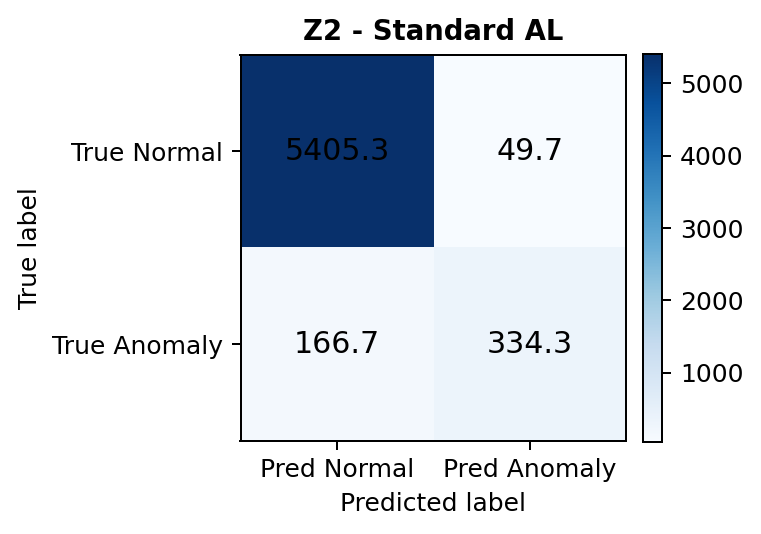
\includegraphics[width=0.42\linewidth]{figs/results/confusion_z2_standard_al.png}%
    \label{fig:cm_z2_std}}
\hfil
\subfloat[Z2---cAL $r^{+} = 4$ (FNR = 0.071, Recall = 0.929)]{%
    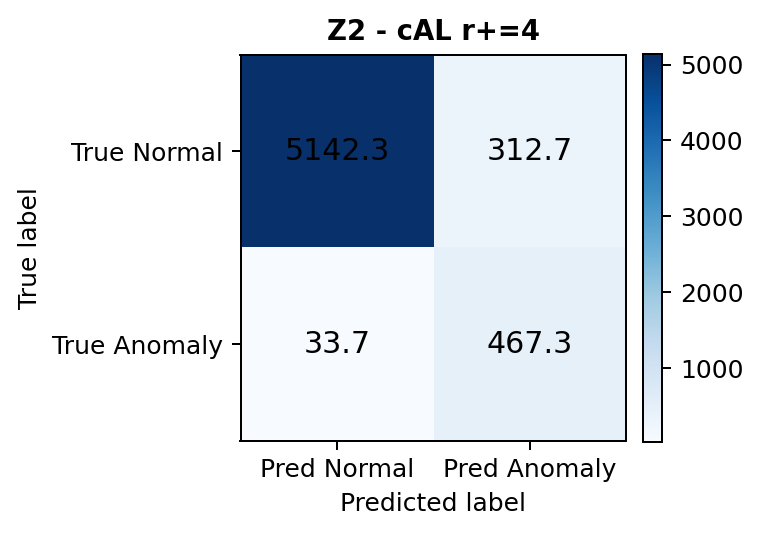
\includegraphics[width=0.42\linewidth]{figs/results/confusion_z2_cal_rp4.png}%
    \label{fig:cm_z2_cal}}
\\
\subfloat[E2---Standard AL (FNR = 0.407, Recall = 0.593)]{%
    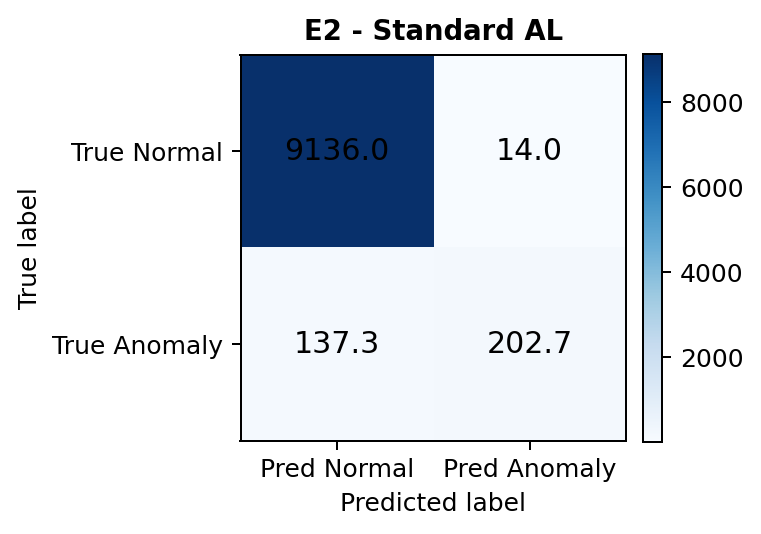
\includegraphics[width=0.42\linewidth]{figs/results/confusion_e2_standard_al.png}%
    \label{fig:cm_e2_std}}
\hfil
\subfloat[E2---cAL $r^{+} = 4$ (FNR = 0.144, Recall = 0.856)]{%
    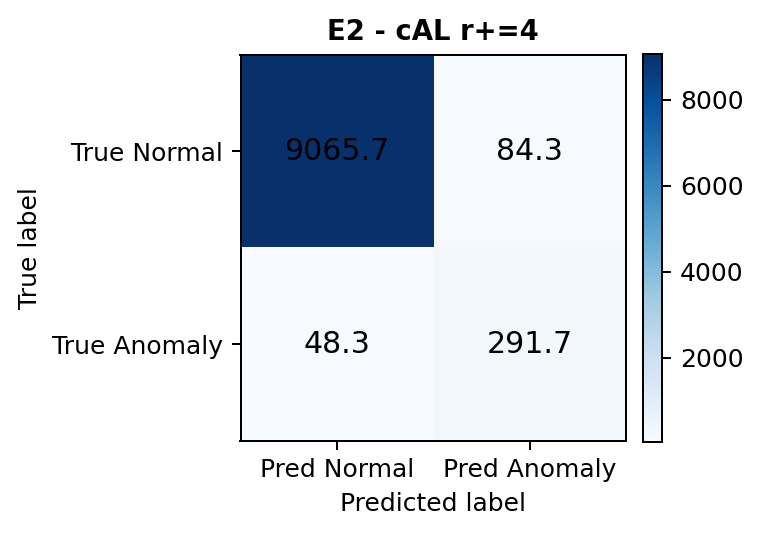
\includegraphics[width=0.42\linewidth]{figs/results/confusion_e2_cal_rp4.png}%
    \label{fig:cm_e2_cal}}
\caption{Scene-level confusion matrices for the two most challenging
scenes at the final annotation budget (representative single run).
Left column: Standard AL. Right column: proposed cAL ($r^{+}=4$).
Mean values over 3 runs: In Scene~Z2, false negatives decrease from
179.9 to 35.6 ($80.2\%$ reduction) and recall increases from $0.641$
to $0.929$. In Scene~E2, false negatives decrease from 138.4 to 49.0
($64.6\%$ reduction) and recall increases from $0.593$ to $0.856$.
These scenes exhibit the highest class imbalance and spectral overlap
in the dataset, making them the most operationally critical for
anomaly detection.}
\label{fig:cm_scene}
\end{figure*}

% ============================================================
%  Anomaly Detection Maps
% ============================================================

\subsection{Spatial Anomaly Detection Maps}

Fig.~\ref{fig:anomaly_maps} provides a spatial visualisation of the
detection outcomes for the two most challenging scenes, Z2 and E2,
at the final annotation budget of 600 labeled superpixels. Each map
overlays the detection result on the false-colour (NIR/R/G) composite:
green regions indicate correctly detected anomalies (TP), red regions
indicate missed anomalies (FN), and blue regions indicate false alarms
(FP); uncoloured areas correspond to correctly identified background (TN).

\begin{figure*}[t]
    \centering
    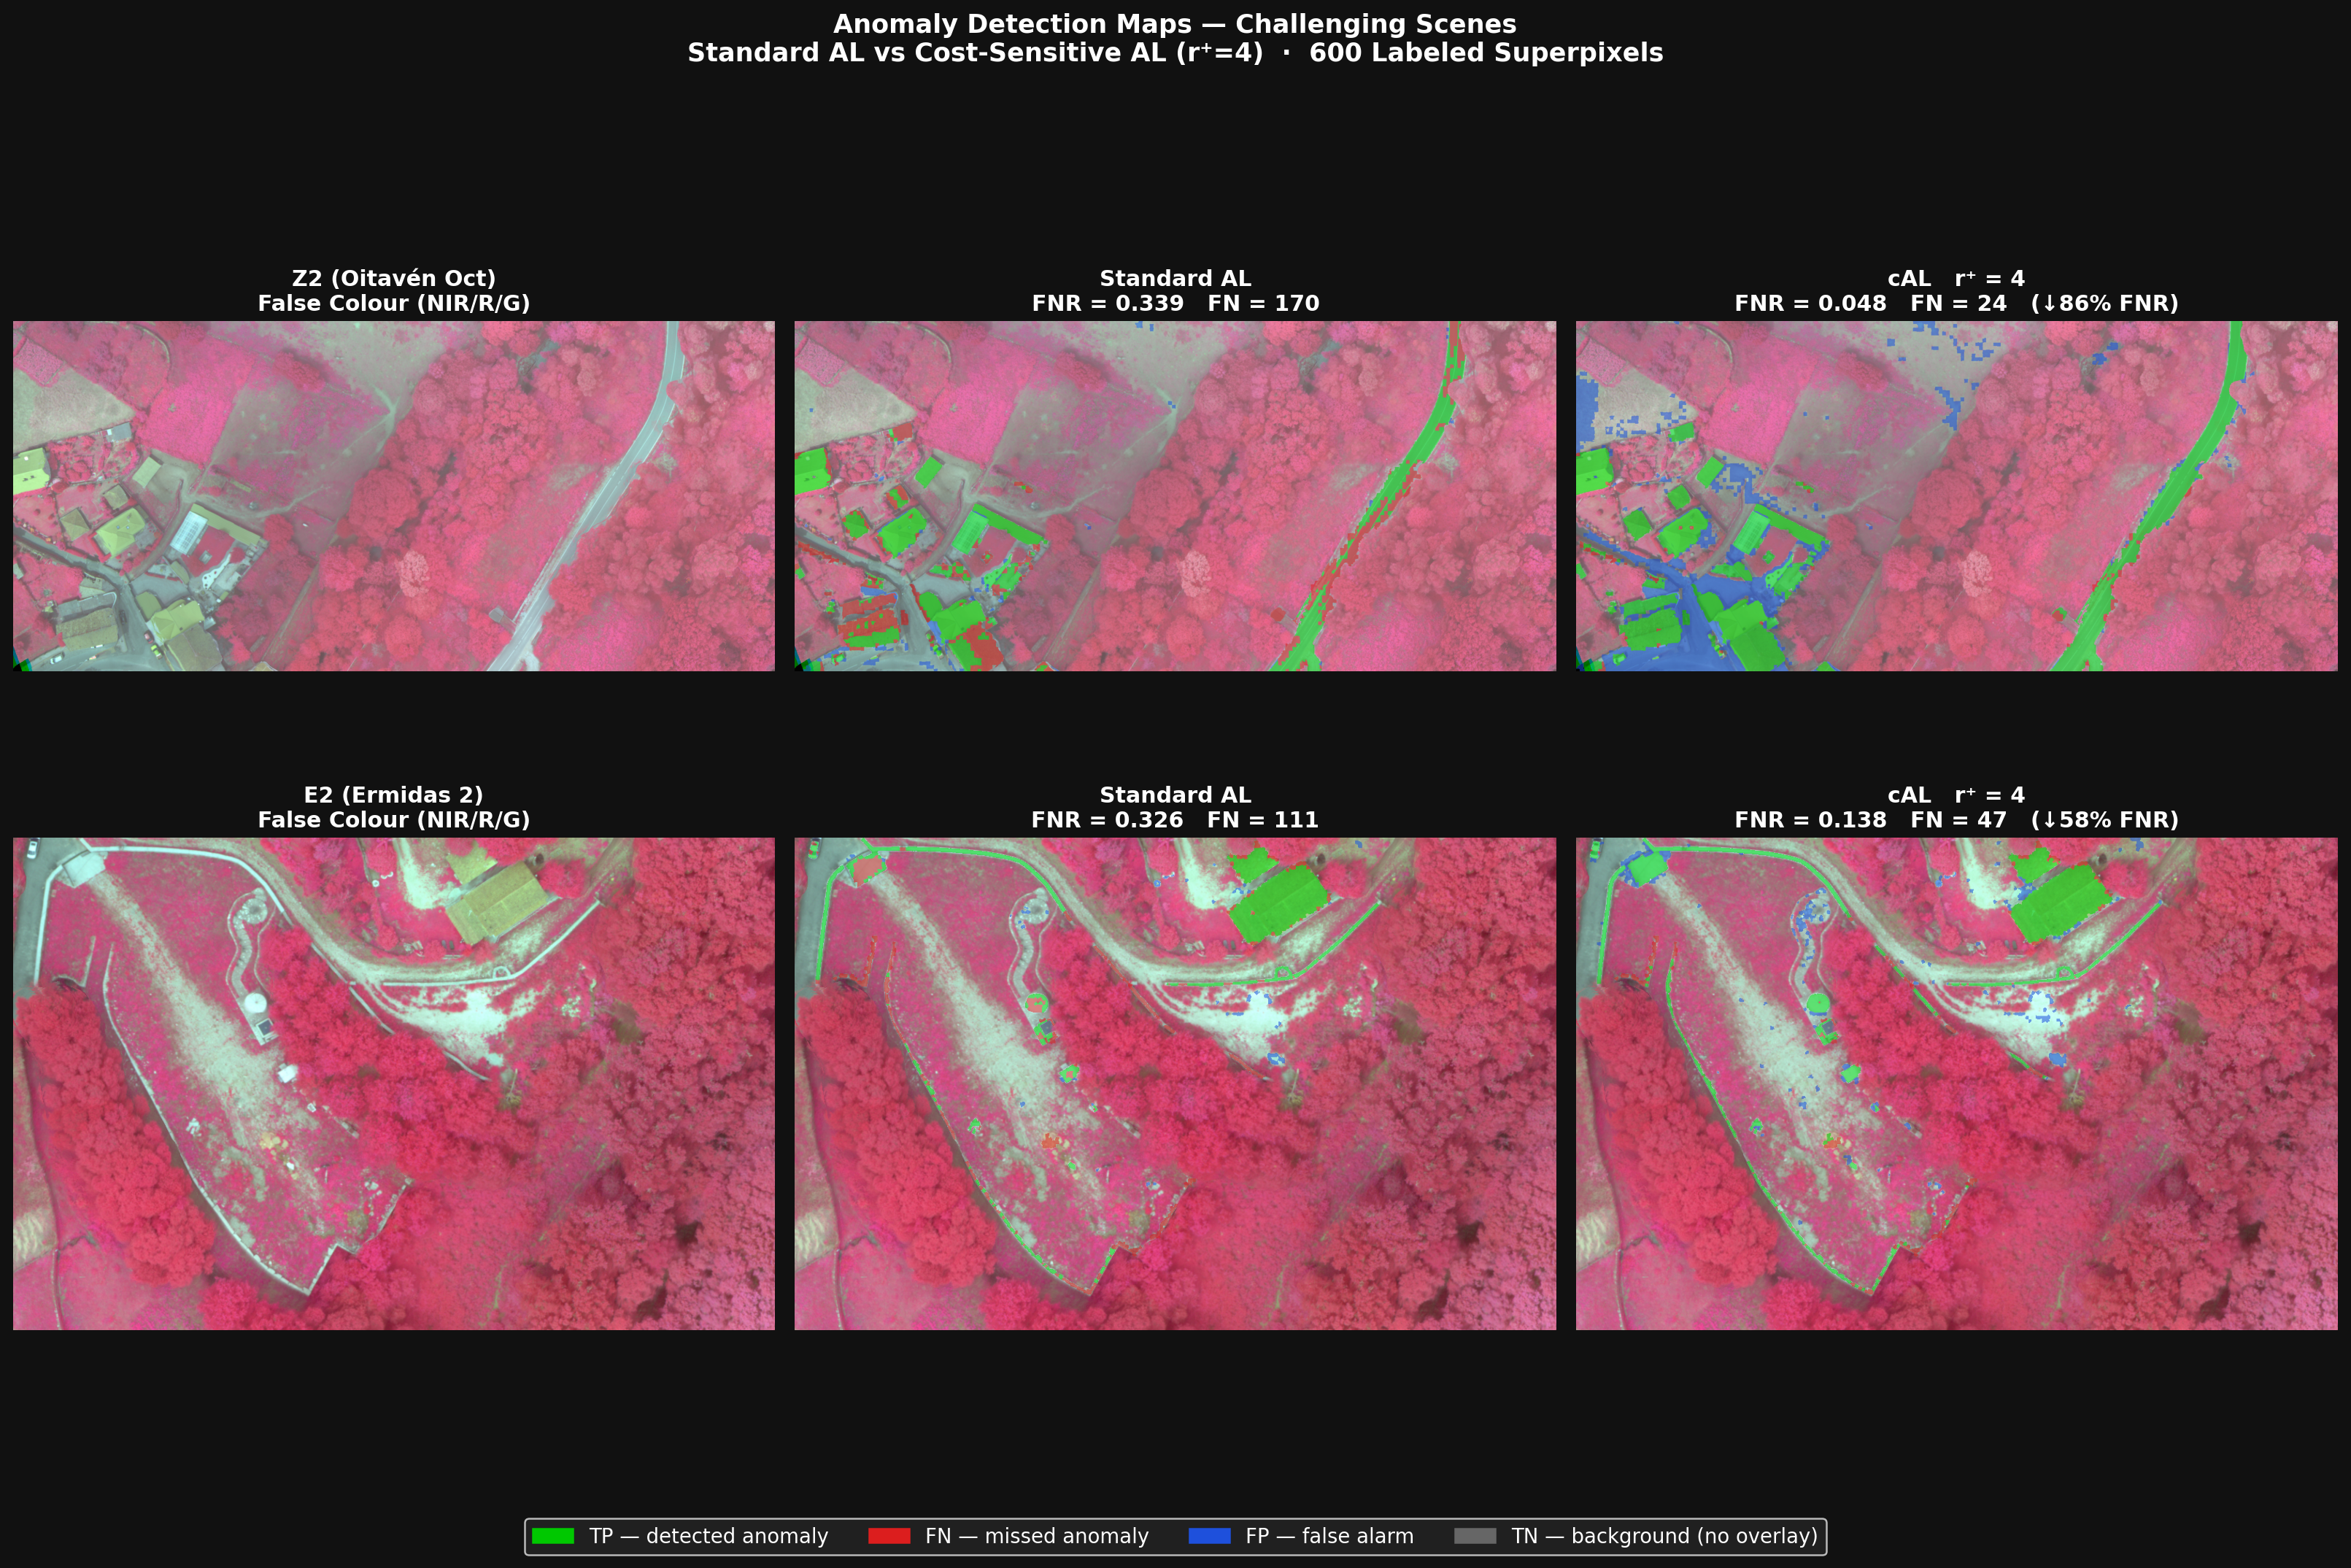
\includegraphics[width=\textwidth,keepaspectratio]{figs/results/anomaly_maps_z2_e2.png}
    \caption{Pixel-level anomaly detection maps for scenes Z2 (top) and
    E2 (bottom) at the final annotation budget (600 labeled superpixels;
    representative single run). Left: false-colour composite (NIR/R/G).
    Centre: Standard AL —
    Z2 FNR\,=\,0.359 (mean over 3 runs), E2 FNR\,=\,0.407.
    Right: cAL ($r^{+}=4$) — Z2 FNR\,=\,0.071 ($\downarrow$80\%),
    E2 FNR\,=\,0.144 ($\downarrow$65\%).
    Green\,=\,TP (detected anomaly); Red\,=\,FN (missed anomaly);
    Blue\,=\,FP (false alarm); background\,=\,TN.}
    \label{fig:anomaly_maps}
\end{figure*}

The spatial maps confirm the quantitative results and reveal the
operational character of the improvement. In Scene~Z2, Standard AL
fails to detect large contiguous anomalous structures (buildings and
roads), leaving substantial red regions across the scene. The cAL
map shows these same structures recovered in green, with only minor
residual red patches, while the blue (FP) overlay remains localised
to boundary regions between vegetation and built-up areas. Scene~E2
exhibits a similar pattern: Standard AL misses dispersed anomalous
structures throughout the riparian corridor, whereas cAL recovers
the majority of these regions. The spatial distribution of false
positives in the cAL maps is consistent with the theoretically
anticipated precision--recall trade-off: the shifted decision boundary
increases anomaly recall at the cost of a controlled increase in false
alarms, predominantly at the spectral transition zones between
anomalous and normal classes.

% ============================================================
%  Feature Set Ablation
% ============================================================

\subsection{Feature Set Ablation}
\label{sec:ablation}

Table~\ref{tab:ablation} evaluates the contribution of the full 19-dimensional
feature representation by running cAL ($r^{+}=4$) with three progressively
richer feature sets under otherwise identical conditions.
\textit{Raw-5D} uses only the five per-superpixel band means;
\textit{Raw-10D} augments these with per-band standard deviations;
\textit{Full-19D} (proposed) additionally incorporates vegetation indices
(NDVI, NDRE, ExG, EVI, BNDVI), spectral band ratios (R/B, NIR/R,
NIR/RedEdge), and a Mahalanobis-like spectral anomaly score
(Section~\ref{sec:feature-extraction}).

\begin{table}[t]
\footnotesize
\centering
\caption{Feature Set Ablation: FNR ($\downarrow$) at Final Budget---cAL ($r^{+}=4$).
         Bold denotes the lowest FNR per scene.}
\begin{tabular}{l r r r r}
    \toprule
    \textbf{Feature Set} & \textbf{Z1} & \textbf{Z2} & \textbf{E1} & \textbf{E2} \\
    \midrule
    Raw-5D  (5 feat.)    & 0.074 & 0.099 & 0.031 & 0.144 \\
    Raw-10D (10 feat.)   & \textbf{0.070} & 0.056 & \textbf{0.023} & 0.105 \\
    Full-19D (proposed)  & 0.072 & \textbf{0.043} & 0.024 & \textbf{0.096} \\
    \bottomrule
\end{tabular}
\label{tab:ablation}
\end{table}

The ablation reveals a scene-dependent benefit pattern. In Scenes~Z1 and E1,
which exhibit low anomaly prevalence and high spectral separability, all three
feature sets yield similar FNR values ($\leq\!0.074$), indicating that the
five-band means are sufficient when the decision boundary is easy to locate
and class imbalance is moderate. In contrast, Scenes~Z2 and E2, characterised
by higher class imbalance and greater within-class spectral variability, show
clear and monotone improvements as the feature space expands. In Scene~Z2,
FNR decreases from $0.099$ (Raw-5D) to $0.056$ (Raw-10D) to $\mathbf{0.043}$
(Full-19D), a cumulative reduction of $56.6\%$ relative to the five-band
baseline. The largest single step is the 5D\,$\to$\,10D transition, which
captures per-superpixel spectral variance---a discriminator for the
heterogeneous texture of anthropogenic structures embedded in riparian
vegetation. The subsequent 10D\,$\to$\,19D step refines further via
vegetation-index and ratio features that amplify the contrast between
photosynthetically active canopy and spectrally anomalous surfaces.
Scene~E2 follows the same monotone trend ($0.144 \to 0.105 \to 0.096$).
These results confirm that the extended feature set is not redundant:
its value is concentrated in the scenes where the anomaly detection task
is most challenging.

% ============================================================
%  V. DISCUSSION
% ============================================================
\clearpage
\section{Discussion}

\subsection{Mechanisms of False-Negative Reduction}

The false-negative reduction observed in Section~IV follows directly
from the design described in Section~III-B: the cSVM shifts the
decision boundary toward the normal class (reducing false negatives
at the cost of additional false positives), the risk-sensitive
uncertainty score~(\ref{eq:uncertainty}) directs query effort toward
the anomaly side of the boundary, and kernel $k$-means diversity
filtering avoids redundant annotation of homogeneous normal regions.
The synergy between these three components explains why cAL
consistently outperforms Unc+KernelKMeans: diversity filtering alone
is insufficient without a cost-sensitive training objective.

\subsection{Interpretation of the Risk Trade-Off}

The results confirm the expected precision--recall trade-off: as $r^{+}$
increases, cAL recovers more anomalies at the cost of additional false
positives. At $r^{+}=4$, aggregate false positives increase from 212.3
(Standard AL) to 762.0 ($+259\%$), while false negatives fall from
515.0 to 174.6 ($-66.1\%$). Because anomalies constitute only
$3\%$--$13\%$ of each scene, the absolute false-positive rate remains
low even after this increase; operationally, each false positive
triggers only a low-cost follow-up inspection, whereas a missed
anomaly may lead to irreversible ecological damage. The appropriate value of $r^{+}$ therefore
depends on the relative cost of inspection vs.\ remediation in the
specific application, and practitioners can tune this coefficient to
reflect their operational requirements. At $r^{+}=2$ and $r^{+}=3$,
cAL already delivers meaningful false-negative reductions (Table~\ref{tab:confusion_scene})
with more moderate false-positive increases, offering a flexible
operating range.

\subsection{Limitations of Symmetric Evaluation Metrics}

A recurring observation in the results is that Standard AL can achieve
comparable or even superior accuracy to cAL while maintaining substantially
higher false-negative rates. This is a direct consequence of class
imbalance: the anomaly class constitutes only 3\%--13\% of each scene,
so a classifier that misses many anomalies still achieves high accuracy.
The risk-weighted cost $C(r^{+})$ makes this failure mode visible by
amplifying the contribution of false negatives to the overall error.
The confusion-matrix comparison in Fig.~\ref{fig:cm_scene} illustrates
this starkly: Standard AL appears competitive on aggregate accuracy
metrics but leaves 515.0 anomalies undetected, compared with 174.6 for
cAL. Practitioners relying solely on accuracy or ROC-AUC to select an
active learning strategy may, therefore, inadvertently deploy a system with
poor anomaly recall in exactly the scenes that matter most.

\subsection{Limitations and Future Work}

Several limitations of the present study should be acknowledged.
First, the dataset comprises four UAV scenes from a single geographic
region; generalisation to other biomes, sensor configurations, or anomaly
types remains to be evaluated. Second, cAL experiments use three repeated
runs due to computational cost; bootstrap confidence intervals over a
larger number of repetitions would strengthen statistical reliability.
Third, the current framework applies a fixed $r^{+}$ throughout the
active learning trajectory; an adaptive schedule that decreases $r^{+}$
as recall improves could improve the precision--recall balance at later
budget stages. Fourth, the superpixel feature representation does not
exploit spatial context beyond the immediate superpixel neighbourhood;
graph-based or convolutional representations may improve discriminability
in spatially structured scenes. Fifth, in Scene~E2 the Mahalanobis oracle
classifier (threshold selected on the full labeled pool) achieves a lower
FNR than cAL; however, this classifier relies on complete pool supervision
for threshold calibration and is not a competing active learning method ---
among AL methods, cAL ($r^{+}=4$) remains the best performer in E2 by a
substantial margin. Future work will also explore the
integration of conformal prediction to provide coverage-guaranteed
anomaly detection maps alongside the active learning system.

% ============================================================
%  VI. CONCLUSION
% ============================================================
\section{Conclusion}

This paper presents a cost-sensitive active learning framework for
reducing missed environmental anomalies in UAV multispectral imagery.
The method integrates risk-weighted SVM training, risk-sensitive
uncertainty sampling, and kernel $k$-means diversity filtering into a
unified pool-based active learning loop governed by a single risk
coefficient $r^{+}$. Experiments on four UAV multispectral riparian
scenes show that the proposed approach substantially reduces false
negatives and risk-weighted misclassification cost under limited
labeling budgets, particularly in challenging scenes. The aggregate
confusion-matrix analysis demonstrates a reduction in false negatives
from 515.0 (Standard AL) to 174.6 (cAL, $r^{+}=4$), increasing anomaly
recall from $0.777$ to $0.924$. These findings support risk-sensitive
active learning as a practical strategy for environmental monitoring
scenarios in which missed anomalies are more operationally costly than
additional false alarms.

% ============================================================
%  ACKNOWLEDGMENTS
% ============================================================
\section*{Acknowledgments}
% [Grant acknowledgments and data repository citation.]

% ============================================================
%  REFERENCES
% ============================================================
\bibliographystyle{ieeetr}
\bibliography{bibtex/bib/IEEEabrv,bibliography}

% ============================================================
%  BIOGRAPHY SECTION
% ============================================================
\clearpage   % flush all pending floats before biographies

\begin{IEEEbiography}[{\includegraphics[width=1in,height=1.25in,clip,keepaspectratio]{ali.png}}]{Ali G{\"u}ne\c{s}}
received the B.Sc., M.Sc., and Ph.D.\ degrees in computer engineering from S{\"u}leyman Demirel University, Isparta, Turkey, in 2009, 2012, and 2017, respectively. His doctoral research was carried out at the Remote Sensing Laboratory, University of Trento, Trento, Italy, under the supervision of Prof.\ Lorenzo Bruzzone, supported by a T\"{U}B{\.I}TAK 2214-A International Research Fellowship. He is currently a faculty member with the Department of Software Engineering, Faculty of Engineering and Natural Sciences, Istanbul Atlas University, Istanbul 34406, Turkey.

His research interests include hyperspectral image processing and classification, remote sensing, machine learning, deep learning, and pattern recognition.

Dr.\ G{\"u}ne\c{s} is the author of several peer-reviewed articles in journals including \textit{Land}, \textit{Expert Systems with Applications}, \textit{Signal, Image and Video Processing}, and \textit{IEEE Journal of Selected Topics in Applied Earth Observations and Remote Sensing}. He serves as a reviewer for the \textit{IEEE Transactions on Industrial Electronics}, the IEEE International Conference on Image Processing Theory, Tools and Applications (IPTA), and the Signal Processing and Communications Applications Conference (SIU).
\end{IEEEbiography}

% TODO: Replace "Author Two" with the real name and add photo before submission.
% Affiliation: Department of Electronics and Computer Science,
%              Universidade de Santiago de Compostela, 15782 Spain
\begin{IEEEbiographynophoto}{Author Two}
% [Fill in before submission]
received the [degree] from [university], [city], [country], in [year].
He/She is currently with the Department of Electronics and Computer Science,
Universidade de Santiago de Compostela, 15782 Santiago de Compostela, Spain
(e-mail: author@usc.es).
[Research interests.]
\end{IEEEbiographynophoto}

% TODO: Replace "Author Three" with the real name and add photo before submission.
\begin{IEEEbiographynophoto}{Author Three}
% [Fill in before submission]
received the [degree] from [university], [city], [country], in [year].
He/She is currently with the Department of Electronics and Computer Science,
Universidade de Santiago de Compostela, 15782 Santiago de Compostela, Spain
(e-mail: author@usc.es).
[Research interests.]
\end{IEEEbiographynophoto}

\vfill
\end{document}
